\documentclass[../notas medios.tex]{subfiles}
\begin{document}

\chapter{Análisis de Deformaciones}

\graphicspath{{IMAGES/Cap5/}} 								 % Specifies the directory where pictures are stored
\section{Introducción}

Al final de esta sección el estudiante deberá estar en la capacidad de:

\begin{itemize}
\item[•] Reconocer la diferencia entre desplazamientos absolutos y relativos entre los puntos materiales.
\item[•] Entender los cambios geométricos impartidos al aplicar una transformación líneal sobre un campo vectorial.
\item[•] Identificar los efectos físicos contenidos en el tensor de deformaciones infinitesimales.
\item[•] Calcular el tensor de deformaciones infinitesimales a partir del campo de desplazamientos relativos. 
\item[•] Reconocer la diferencia entre la configuración deformada de un medio continuo y la deformada del punto material
\end{itemize}

Del análisis de las fuerzas “internas” se concluyó, -vía aplicación de las 3 leyes de Newton sobre un volumen arbitrario de un medio continuo-, que estas corresponden a nivel local a una función (continua) de carácter tensorial y que satisface el problema de valores en la frontera especificado por las ecuaciones de equilibrio (leyes generalizadas de Newton) y la asignación de las tracciones en la superficie del medio (\cref{equtr_5}, \cref{equrot_5}):

\begin{equation} \label{equtr_5}
\begin{split}
& \frac{{\partial {\sigma _{xx}}}}{{\partial x}} + \frac{{\partial {\tau _{yx}}}}{{\partial y}} + \frac{{\partial {\tau _{zx}}}}{{\partial z}} + {B_x} = 0 \\
& \frac{{\partial {\tau _{xy}}}}{{\partial x}} + \frac{{\partial {\sigma _{yy}}}}{{\partial y}} + \frac{{\partial {\tau _{zy}}}}{{\partial z}} + {B_y} = 0 \\
& \frac{{\partial {\tau _{xz}}}}{{\partial x}} + \frac{{\partial {\tau _{yz}}}}{{\partial y}} + \frac{{\partial {\sigma _{zz}}}}{{\partial z}} + {B_z} = 0 
\end{split}
\end{equation}

\begin{equation} \label{equrot_5}
\begin{split}
& \tau _{xy} = {\tau _{yx}} \\
& \tau _{xz} = {\tau _{zx}} \\
& \tau _{yz} = {\tau _{zy}}
\end{split}
\end{equation}

Se dispone de 6 ecuaciones en 9 incógnitas controlando la distribución espacial de las fuerzas internas $\sigma$ sobre los diferentes puntos materiales del medio continuo.  Dichas fuerzas internas son generadas ya sea por las fuerzas de superficie (tracciones) ${{\vec t}^{(\hat n)}}$  y/o por las interacciones a distancia o fuerzas de cuerpo ${\vec B}$.  Sin embargo, en este punto el problema se hace (matemáticamente) indeterminado ya que se dispone de más incógnitas que ecuaciones.

La indeterminación desde el punto de vista de fuerzas no debe ser para nada sorpresiva, ya que si éstas se consideran como las “funciones causa” es claro que aún falta por involucrar los efectos o “funciones respuesta”. Estas funciones corresponden precisamente a los cambios (cinemáticos) o de configuración, experimentados por las infinitas partículas una vez son sometidas a interacciones externas.

Claramente se identifica la primera necesidad de estudiar los cambios de configuración como la de tratar de establecer una conexión entre estos cambios y las fuerzas internas $\sigma$ y que permita a la postre eliminar la indeterminación matemática del problema de valores en la frontera (PVF) (especificado por las \cref{equtr_5} y \cref{equrot_5}).

Aunque es claro que las nuevas configuraciones aparecen debidas a los desplazamientos a los que son sometidas las diferentes partículas, a la hora de establecer la conexión entre éstas y las fuerzas internas $\sigma$ es importante considerar que son en realidad los desplazamientos relativos  quienes generan estas fuerzas internas.  La aparición de desplazamientos relativos necesariamente se reflejará en términos de cambios de forma  del medio continuo.

\subsection{Concepto intuitivo de deformación}
La \cref{viga1} muestra, en sombreado gris, una viga en voladizo en su configuración original (antes de aplicar las cargas externas) y en línea punteada su configuración final (o deformada)\footnote{En la configuración deformada los puntos materiales o elementos constitutivos de la viga estarán sometidos a un estado de tensiones que satisface las ecuaciones de equilibrio local ( a nivel diferencial) y global.} resultante tras aplicar alguna distribución de cargas externas en forma de tracciones.

Como resultado de la aplicación de las cargas externas los puntos materiales que conforman la viga experimentan desplazamientos. En lo que sigue denominaremos campo de desplazamientos a la variación espacial de estos, y lo denotaremos como $\vec u(\vec x)$. Tal y como se aprecia de manera intutitiva, los desplazamientos varían para los diferentes puntos de la viga generándose \textbf{\textit{desplazamientos relativos}}.

\begin{figure}[H]
\centering
	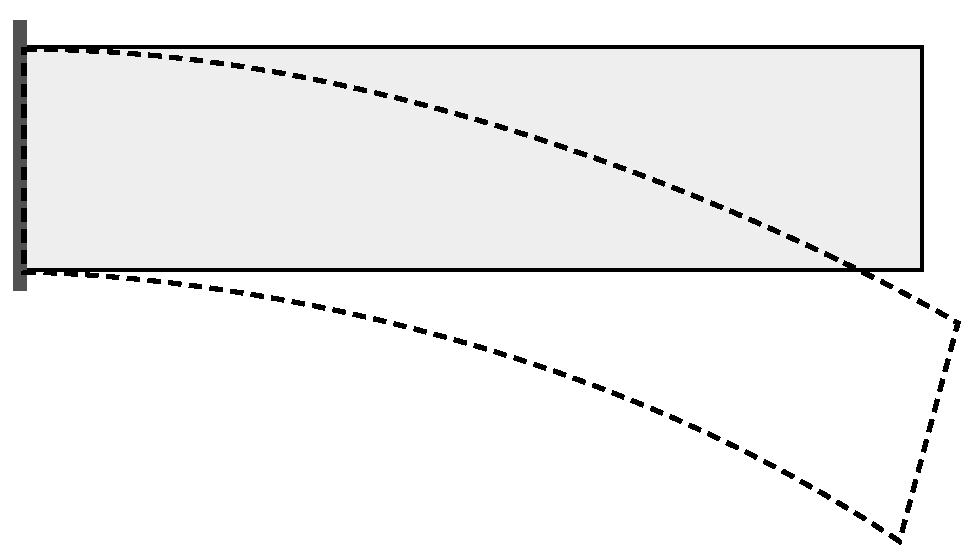
\includegraphics[width=2.5 in]{Fig1.pdf}
	\caption{Configuración original y deformada de una viga en voladizo.}
	\label{viga1}
\end{figure}


Por ejemplo, es evidente que los desplazamientos sobre el empotramiento son "nulos" mientras que los puntos cercanos al extremo derecho de la viga experimentan los máximos desplazamientos. Sin embargo, sabemos que las fuerzas internas (o tensiones) están ligadas al desplazamiento relativo entre los puntos materiales. El propósito de esta sección es hacer una descripción local (o diferencial) de los desplazamientos relativos entre puntos materiales y que pueda ser conectada posteriormente con el tensor de tensiones a través de propiedades de los materiales . Con esto, no solo se conseguirá completar las ecuaciones para el problema de valores en la frontera del medio continuo, sino que además será posible describir la nueva configuración del medio, resultante de la apicación de interacciones externas tanto a nivel local (diferencial) como global.

Para aclarar, nuevamente de manera intuitiva, el caracter local de los cambios relativos la \cref{steady_state} muestra la configuración original (\cref{nodef}) y deformada (\cref{sidef}) de la viga en voladizo. Como elemento auxiliar de análisis esta vez se ha dibujado una rejilla de elementos perfectamente cuadrados sobre la configuración no-deformada.   Si suponemos que estos elementos son de lado $h$ es claro que en el modelo del continuo el punto material corresponde a uno de estos en el estado limite cuando $h \to 0.$ Es evidente de la \cref{sidef} como los diferentes elementos cambian su forma una vez la viga pasa de la configuración descargada a la cargada. Mas aún es evidente de la misma figura como estos cambios varían de elemento a elemento.

\begin{figure}[H]
     \centering
     \subfloat[Configuración original con elementos diferenciales no deformados]{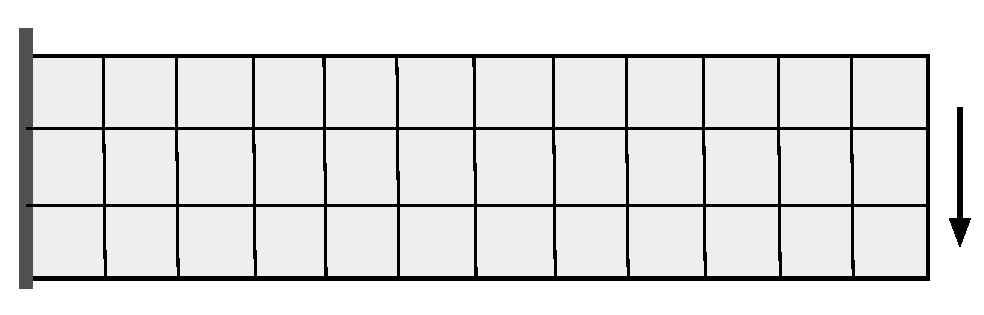
\includegraphics[width=2.8 in]{Fig2a.pdf}\label{nodef}}
     \hspace{0.5cm}\\
     \subfloat[Configuración final con elementos diferenciales deformados]{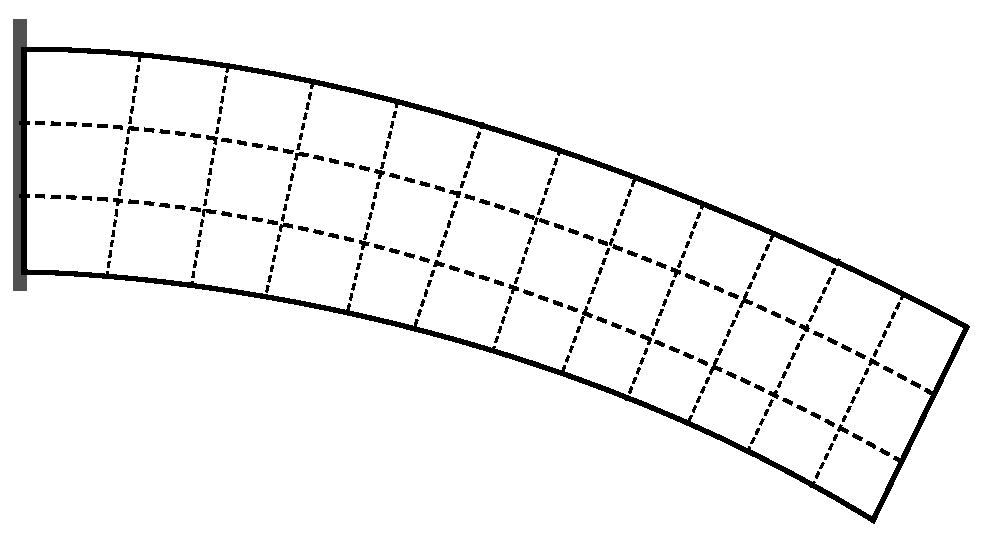
\includegraphics[width=2.8 in]{Fig2b.pdf}\label{sidef}}
     \caption{Comparción entre configuración original y deformada con elementos diferenciales.}
     \label{steady_state}
\end{figure}

La \cref{viga3} muestra nuevamente ambas configuraciones y sobre estas se han seleccionado para efectos ilustrativos dos elementos localizados sobre el empotramiento y sobre el extremo libre del voladizo. En la configuración original ambos elementos son identicos y corresponden a cudrados de lado $h$. En la configuración deformada, mostrada con líneas punteadas, se resaltan nuevamente estos 2 elementos de donde se pueden hacer las siguientes observaciones:

El elemento sobre la parte superior del empotramiento experimenta cambios de tamaño y de forma a través de alargamientos en la dirección longitudinal, mientras que el elemento sobre la parte inferior experimenta acortamientos igualmente en la dirección longitudinal. Estos cambios suceden a pesar de que dichos elementos se encuentran sobre el empotramiento donde los desplazamientos como tal son nulos. De otro lado, el elemento sobre el extremo libre de la viga experimenta pequeños cambios de forma  (no apreciables en el dibujo) y experimentan las mayores rotaciones como si fuera un cuerpo rigido. Los pequeños cambios de forma son equivalentes a pequeños desplazamientos relativos aunque estos puntos experimentan los mayores desplazamientos absolutos.


\begin{figure}[H]
\centering
	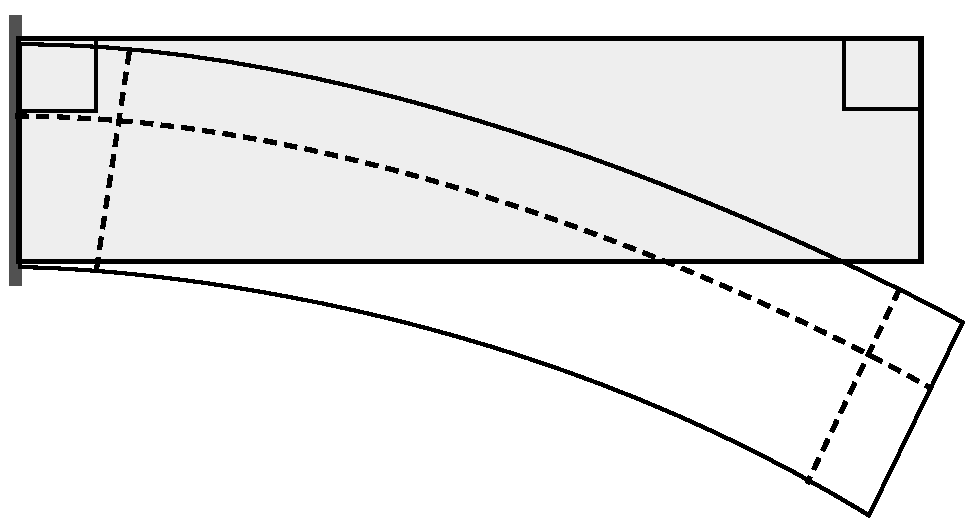
\includegraphics[width=2.5 in]{Fig3.pdf}
	\caption{Elementos con máxima deformación y máxima rotación.}
	\label{viga3}
\end{figure}

En resumen, el propósito de esta sección es hacer una descripción local (o diferencial) de los desplazamientos relativos entre los puntos materiales de un medio continuo cuando este es sometido a la acción de fuerzas externas. En general, como se verá mas adelante, estos cambios se describirán en términos de cambios de tamaño (o magnitud) y de orientación de las "fibras materiales" que emanan de la partícula en las diferentes direcciones tal y como se esquematiza en la \cref{fibras}. Esta muestra un punto material de un medio continuo conjuntamente con su vecindad matemática representada por fibras imaginarias de material, mostradas en líneas punteadas. En la figura el punto material en estudio se muestra con relleno de color negro y se denomina $P$. Adicionalmente se muestra un punto material arbitrario (sin relleno) y denominado $P'$.En el lado izquierdo se muestra la localización de ambos puntos materiales en un instante de tiempo $t=0$, correspondiente a la configuración original o descargada. Tras la aplicación de las cargas ambos puntos materiales se desplazan a las posiciones señaladas como $Q$ y $Q'$ respectivamente y mostradas en lado derecho de la figura correspondiente a un instante de tiempo $t=t$. Como resultado de los desplazamientos experimentados por los puntos materiales la fibra material que une los mismos experimenta cambios de tamaño y de orientación.

\begin{figure}[H]
\centering
	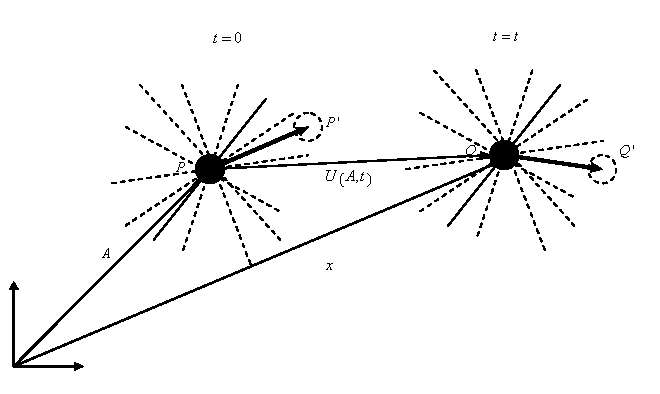
\includegraphics[width=4.0 in]{fibras.pdf}
	\caption{Fibras materiales en la configuración original y deformada.}
	\label{fibras}
\end{figure}

En lo que sigue estudiaremos la relación entre 2 fibras arbitrarias como las mostradas en la figura desde 2 puntos de vista. Inicialmente se estudiarán los cambios de magnitud y orientación experimentados por un vector posición tras operarlo con una matriz conservando la propiedad de línealidad. Posteriormente estudiaremos el problema a nivel infinitesimal tras analizar un par de puntos, unidos por una fibra material de tamaño diferenial. Dicho analisis permitirá encontrar el tensor graiente de desplazamientos como medida local (o diferencial) de la deformación\footnote{Aunque hasta el momento el tratamiento del medio continuo no ha especificado ninguna diferencia entre medios sólidos, liquidos o gases el tratamiento cinematico que se presenta si esta restringido al caso de pequeñas deformaciones}.


\section{Transformaciones lineales}
Con el propósito de conceptualizar el proceso deformación o cambios de configuración a nivel local o diferencial es conveniente apoyarnos como herramienta de análisis en las transformaciones lineales\footnote{Esta sección esta basada en los textos: Principles of Solid Mechanics. Rowland Richards Jr. CRC Press, 2001 y Introduction to the Mechanics of Continuous Medium. Lawrence E Malvern. Prentice Hall, 1969.}. En términos simples estas corresponden a la traformación de un vector en otro conservando la propiedad de línealidad. Esta idea se ilustra en la \cref{amat} en la que $\vec r = {r_x}\hat i + {r_y}\hat j$ representa el vector posición de un punto $P$. Como resultado de alguna acción externa, representada por un tensor $A$ este punto material experimenta un desplazamiento $\vec \Delta  = {\Delta _x}\hat i + {\Delta _y}\hat j$ con lo que que el vector $\vec{r}$ se transforma en el vector $\vec \rho  = {\rho _x}\hat i + {\rho _y}\hat j$. Esta relación puede escribirse como:

\begin{equation}
\vec \rho  = A \cdot \vec r
\label{amat}
\end{equation}

%
\begin{figure}[H]
\centering
	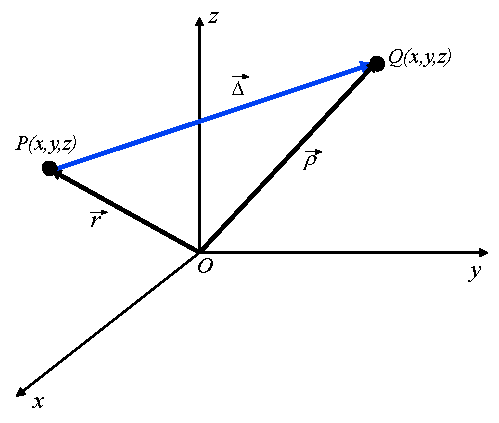
\includegraphics[width=3.0 in]{trans.pdf}
	\caption{Transformación del vector $\vec{r}$ en el vector $\vec{\rho}$.}
	\label{trans}
\end{figure}

El vector $\vec{r}$ al transformarse en el vector $\vec{\rho}$ experimenta 2 tipos de cambios:

\begin{itemize}
\item[i] Cambios de magnitud (o de tamaño).
\item[ii] Cambios de orientación (dirección). 
\end{itemize}

La relación \cref{amat} entre $\vec{r}$ y $\vec{\rho}$ puede escribirse en forma explicita como:

\begin{equation}
\left\{ {\begin{array}{*{20}{c}}
{{\rho _x}}\\
{{\rho _y}}
\end{array}} \right\} = \left[ {\begin{array}{*{20}{c}}
{{a_{xx}}}&{{a_{xy}}}\\
{{a_{yx}}}&{{a_{yy}}}
\end{array}} \right]\left\{ {\begin{array}{*{20}{c}}
{{r_x}}\\
{{r_y}}
\end{array}} \right\}
\label{roaere}
\end{equation}

La \cref{roaere} indica que la matriz $A$ transforma el vector $\vec{r}$ en el vector $\vec{\rho}$ y por ende ésta contiene toda la información referente a los cambios de magnitud y dirección que experimentan las infinitas direcciones que emanan del punto $O$. Una transformación como la descrita en la \cref{roaere} se denomina lineal si satisface la condición dada por:

\begin{equation}
A \cdot \left( {{{\vec r}_1} + {{\vec r}_2}} \right) = A \cdot {{\vec r}_1} + A \cdot {{\vec r}_2}
\label{lineal}
\end{equation}

la cual implica que lineas rectas y paralelas antes de la transformación permanecen rectas y paralelas después de la transformación o en otras palabras que conservan la ley del paralelogramo. Esto se ilustra en la \cref{paralelo}:

\begin{figure}[H]
\centering
	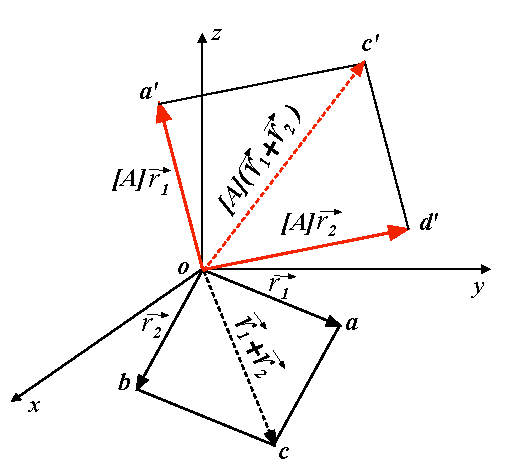
\includegraphics[width=3.0 in]{paralelo.pdf}
	\caption{Definición de línealidad.}
	\label{paralelo}
\end{figure}

Alternativamente, es posible escribir la transformación en términos del vector de desplazamientos ${\vec \Delta }$  que experimenta la cabeza del vector $\vec{r}$ como sigue;  

\[\vec \Delta  = \vec \rho  - \vec r\]

\[\vec \Delta  = A \cdot \vec r - \vec r\]

\[\vec \rho  = \left[ {A - I} \right] \cdot \vec r\]

\[\vec \Delta  = D \cdot \vec r\]

y de manera explicta escribimos;

\begin{equation}
\left\{ {\begin{array}{*{20}{c}}
{{\Delta _x}}\\
{{\Delta _y}}
\end{array}} \right\} = \left[ {\begin{array}{*{20}{c}}
{{d_{xx}}}&{{d_{xy}}}\\
{{d_{yx}}}&{{d_{yy}}}
\end{array}} \right]\left\{ {\begin{array}{*{20}{c}}
{{r_x}}\\
{{r_y}}
\end{array}} \right\}
\label{disp}
\end{equation}

La matriz $D$ se denomina la matriz de transformación de desplazamientos. En lo que sigue estudiaremos transformaciones como las dadas en la \cref{disp} identificando los efectos que dicha matriz impone sobre las diferentes direcciones que emanan de un punto material. 

\subsection{Componente rotacional}
A continuación nos disponemos a estudiar el efecto de los diferentes términos en la matriz de transformación de desplazamientos $D$. Abordemos inicialmente los cambios de orientación impartidos por $D$ en los diferentes vectores. Considerando la \cref{rota}, en esta el vector original $\vec{r}$ se transforma en el vector $\rho$ tras realizar una rotación $\alpha$. 

\begin{figure}[H]
\centering
	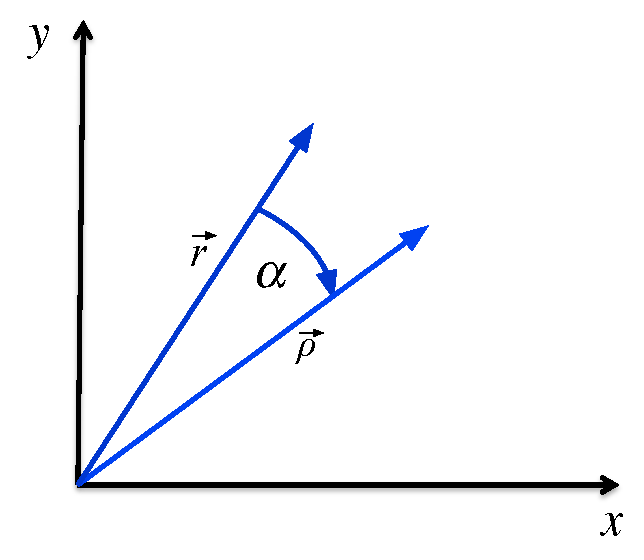
\includegraphics[width=3.0 in]{rota.pdf}
	\caption{Rotación a través de un angulo $\alpha$ del vector $\vec{r}$ en el vector $\vec{\rho}$.}
	\label{rota}
\end{figure}


Relacionando las componentes rectangulares de ambos vectores se tiene que:

\[{\rho _x} = {r_x} + \alpha {r_y}\]
y
\[{\rho _y} = {r_y} - \alpha {r_x}.\]

De manera explicita, pero en términos de los desplazamientos de la cabeza del vector posición $\vec{r}$ lo anterior resulta en:

\begin{equation}
\left\{ {\begin{array}{*{20}{c}}
{{\Delta _x}}\\
{{\Delta _y}}
\end{array}} \right\} = \left[ {\begin{array}{*{20}{c}}
0&\alpha \\
{ - \alpha }&0
\end{array}} \right]\left\{ {\begin{array}{*{20}{c}}
{{r_x}}\\
{{r_y}}
\end{array}} \right\}
\label{asym}
\end{equation}

De la \cref{asym} se concluye que la componente rotacional del tensor de transformación de desplazamientos $D$ es una matriz con $0s$ en la diagonal y términos iguales pero con signo opuesto a uno y otro lado de la diagonal. En el lenguaje del análisis tensorial, extendido en este caso a matrices, a estos tensores se les conoce como tensores anti-simétricos. En conclusión \textbf{\textit{la componente rotacional de la transformación lineal corresponde a un tensor anti-simétrico.}}


\subsection{Componente simétrica}
Como ya ha sido identificado en los planteamientos anteriores, la matriz de transformación de desplazamientos $D$ imparte en las diferentes direcciones cambios de dirección y de magnitud. El haber identificado el efecto rotacional como la componente anti-simétrica de $D$ permite concluir que el término restante, y simétrico por demás, contendrá los efectos asociados a los cambios de tamaño o magnitud de los diferentes vectores. De dicha conclusión resulta natural resolver el tensor $D$ precisamente en una componente simétrica y en una componente anti-simétrica como:


\begin{equation}
\left[ {\begin{array}{*{20}{c}}
{{d_{xx}}}&{{d_{xy}}}\\
{{d_{yx}}}&{{d_{yy}}}
\end{array}} \right] = \left[ {\begin{array}{*{20}{c}}
{{d_{xx}}}&{\frac{{{d_{xy}} + {d_{yx}}}}{2}}\\
{\frac{{{d_{yx}} + {d_{xy}}}}{2}}&{{d_{yy}}}
\end{array}} \right] + \left[ {\begin{array}{*{20}{c}}
0&{\frac{{{d_{xy}} - {d_{yx}}}}{2}}\\
{\frac{{{d_{yx}} - {d_{xy}}}}{2}}&0
\end{array}} \right].
\label{descomp}
\end{equation}

En esta partición es evidente que el segundo término del lado derecho corresponde efectivamente a la componente rotacional del tensor (componente anti-simétrica), mientras que el primer término necesariamente contendrá la información relativa a los cambios de tamaño. Nótese además que este primer término es simétrico con respecto a la diagonal. De forma general escribimos esta partición de la matriz de transformación de desplazamientos $D$ como:


\begin{equation}
D = \varepsilon  + \omega
\label{parti}
\end{equation}

donde $\varepsilon$ contiene los efectos de cambio de tamaño y $\omega$ contiene los efectos de cambio de orientación.

Para estudiar los efectos de las diferentes componentes del tensor de transformación de desplazamientos $D$ usaremos el cuadrado unitario de la \cref{unitario}.

\begin{figure}[H]
\centering
	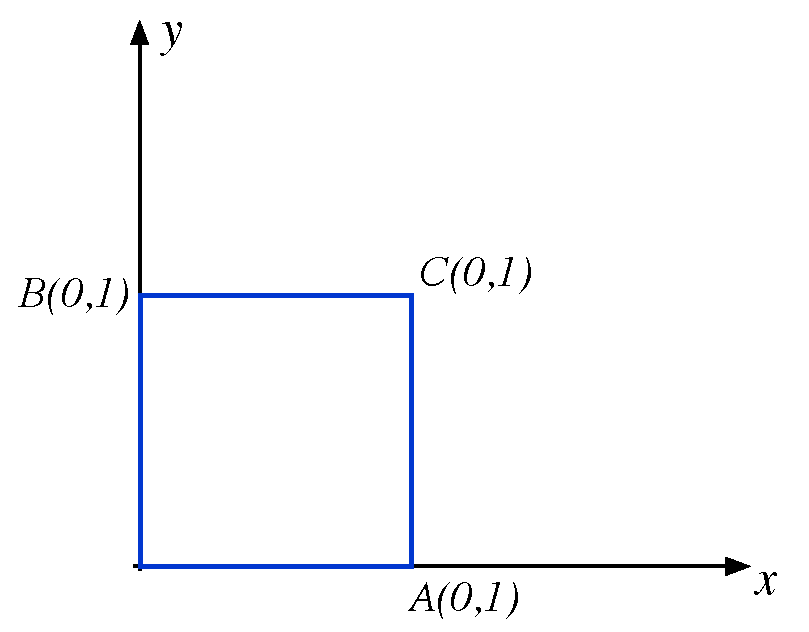
\includegraphics[width=2.0 in]{unitario.pdf}
	\caption{Cuadrado unitario a ser transformado por el tensor $D$.}
	\label{unitario}
\end{figure}

Como método de análisis aplicaremos las diferentes componentes del tensor $D$ sobre los vectores posición de los puntos $A$, $B$ y $C$ dados por:

\[{{\vec r}_A} = 1.0\hat i\]
\[{{\vec r}_B} = 1.0\hat j\]
\[{{\vec r}_C} = 1.0\hat i + 1.0\hat j\]

y asumiremos que los puntos $O$, $A$, $B$ y $C$ permanecen unidos por líneas rectas de acuerdo con la propiedad de linealidad. Posteriormente compararemos la configuración original y deformada del elemento.


Consideremos inicialmente la componente simétrica de la \cref{parti}. Por razones que se harán evidentes más adelante denotemos los elementos de esta componete como:

\[\varepsilon  = \left[ {\begin{array}{*{20}{c}}
{{\varepsilon _{xx}}}&\bar{\gamma} \\
\bar{\gamma} &{{\varepsilon _{yy}}}
\end{array}} \right]\]

Para determinar la configuración deformada aplicamos la expresión:

\[\left\{ {\begin{array}{*{20}{c}}
{\Delta x}\\
{\Delta y}
\end{array}} \right\} = \left[ {\begin{array}{*{20}{c}}
{{\varepsilon _{xx}}}&\bar{\gamma} \\
\bar{\gamma} &{{\varepsilon _{yy}}}
\end{array}} \right]\left\{ {\begin{array}{*{20}{c}}
{{r_x}}\\
{{r_y}}
\end{array}} \right\}\]

a los vectores posición $\vec{r}_A$, $\vec{r}_B$ y $\vec{r}_C$. Esto da como resultado los vectores de desplazamiento:

\[{{\vec \Delta }_A} = {\varepsilon _{xx}}\hat i + \bar{\gamma} \hat j\]
\[{{\vec \Delta }_B} = \bar{\gamma} \hat i + {\varepsilon _{yy}}\hat j\]
\[{{\vec \Delta }_C} = ({\varepsilon _{xx}} +\bar{\gamma}  )\hat i + ({\varepsilon _{yy}} + \bar{\gamma} )\hat j\]

y la configuración deformada mostrada en línea punteada en la \cref{sime}.


\begin{figure}[H]
\centering
	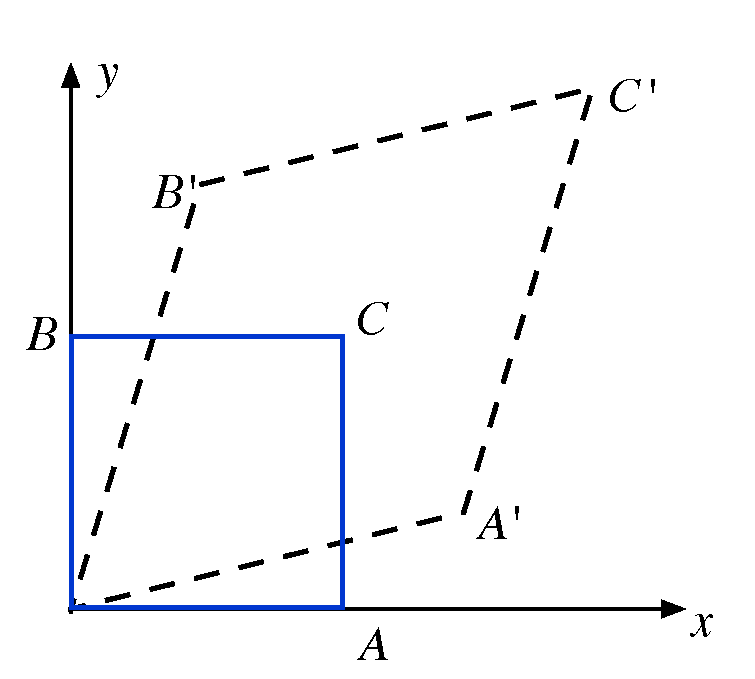
\includegraphics[width=2.5 in]{simetrica.pdf}
	\caption{Configuraciones original y deformada de un cuadrado unitario debido a la componente simétrica $\varepsilon$ del tensor de transformación de desplazamientos $D$.}
	\label{sime}
\end{figure}

\subsection{Componentes escalar y distorsional}
La componente simétrica del tensor de transformación de desplazamientos es análoga al tensor de tensiones estudiado en secciones anteriores. De hecho, dado su caracter simétrico este puede ser estudiado en términos del circulo de Mohr. Identificando esta conexión es posible resolver esta componente en términos adicionales que permiten ahondar en el entendimiento físico del analísis de deformaciones. En particular considere la siguiente descomposición:

\begin{equation}
\left[ {\begin{array}{*{20}{c}}
{{\varepsilon _{xx}}}&\bar{\gamma} \\
\bar{\gamma} &{{\varepsilon _{yy}}}
\end{array}} \right] = \left[ {\begin{array}{*{20}{c}}
{\frac{{{\varepsilon _{xx}} + {\varepsilon _{yy}}}}{2}}&0\\
0&{\frac{{{\varepsilon _{xx}} + {\varepsilon _{yy}}}}{2}}
\end{array}} \right] + \left[ {\begin{array}{*{20}{c}}
{\frac{{{\varepsilon _{xx}} - {\varepsilon _{yy}}}}{2}}&0\\
0&{\frac{{{\varepsilon _{yy}} - {\varepsilon _{xx}}}}{2}}
\end{array}} \right] + \left[ {\begin{array}{*{20}{c}}
0&\bar{\gamma} \\
\bar{\gamma} &0
\end{array}} \right]
\label{otras}
\end{equation}



en la cual se ha separado la componente simétrica en un término escalar (correspondiente al centro del círculo de Mohr) y en 2 términos con información distorsional controlando el radio del círculo. Escribamos la descomposición de $\epsilon$ como:

\[\varepsilon  = pI + S + C\]

donde se reconoce $p={\frac{{{\varepsilon _{xx}} + {\varepsilon _{yy}}}}{2}}$ con lo que el primer término se escribe como:


\[pI = \left[ {\begin{array}{*{20}{c}}
{\frac{{{\varepsilon _{xx}} + {\varepsilon _{yy}}}}{2}}&0\\
0&{\frac{{{\varepsilon _{xx}} + {\varepsilon _{yy}}}}{2}}
\end{array}} \right].\]

Similarmente, haciendo $s = \frac{{{\varepsilon _{xx}} - {\varepsilon _{yy}}}}{2}$ escribimos:


\[S = \left[ {\begin{array}{*{20}{c}}
{\frac{{{\varepsilon _{xx}} - {\varepsilon _{yy}}}}{2}}&0\\
0&{\frac{{{\varepsilon _{yy}} - {\varepsilon _{xx}}}}{2}}
\end{array}} \right] \equiv \left[ {\begin{array}{*{20}{c}}
s&0\\
0&{ - s}
\end{array}} \right]\]

y finalmente

\[C = \left[ {\begin{array}{*{20}{c}}
0&\bar{\gamma} \\
\bar{\gamma} &0
\end{array}} \right].\]

Para entender el efecto físico de cada uno de estos términos aplicaremos nuevamente la transformación al cuadrado unitario previamente definido.

La componente escalar $pI$ genera los siguientes vectores de desplazamientos tras aplicar la \cref{disp}:

\[{{\vec \Delta }_A} = p\hat i\]
\[{{\vec \Delta }_B} = p\hat j\]
\[{{\vec \Delta }_C} = p\hat i + p\hat j\]

resultando en el cambio de forma mostrado en la \cref{scala}

\begin{figure}[H]
\centering
	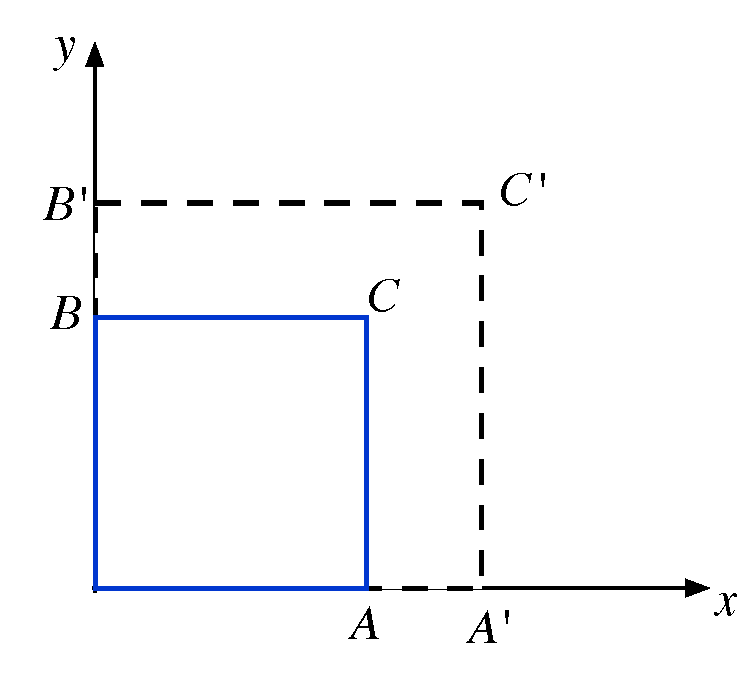
\includegraphics[width=2.5 in]{scala.pdf}
	\caption{Configuraciones original y deformada de un cuadrado unitario debido a la componente escalar de la componente simétrica del tensor de transformación de desplazamientos.}
	\label{escalar}
\end{figure}

De manera similar, la primera componente distorsional $S$ genera los siguientes vectores de desplazamientos:

\[{{\vec \Delta }_A} = s\hat i\]

\[{{\vec \Delta }_B} =  - s\hat j\]

\[{{\vec \Delta }_C} = s\hat i - s\hat j\]

resultando en el cambio de forma mostrado en la \cref{disto1}.

\begin{figure}[H]
\centering
	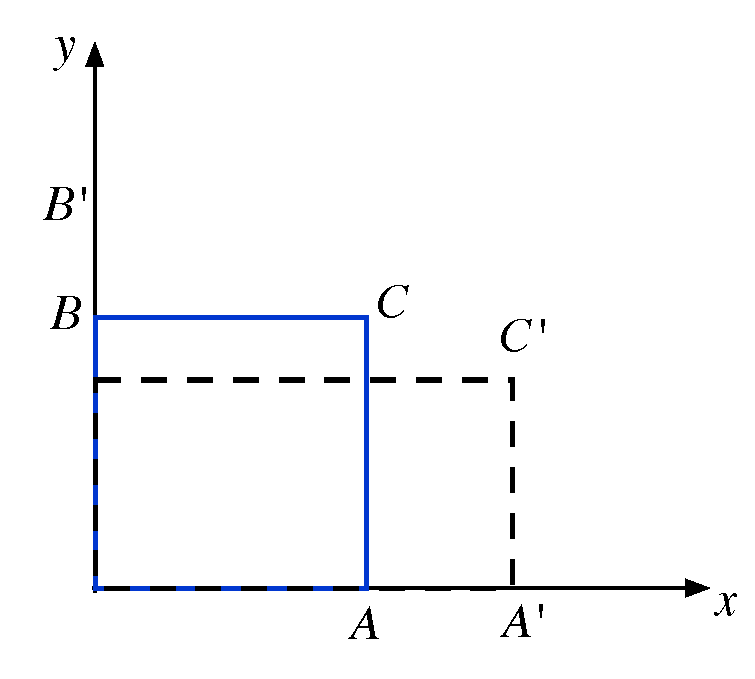
\includegraphics[width=2.5 in]{disto1.pdf}
	\caption{Configuraciones original y deformada de un cuadrado unitario debido a la primera componente distorsional de la componente simétrica del tensor de transformación de desplazamientos.}
	\label{disto1}
\end{figure}

Luego, aplicando la segunda componente distrosional $C$ da como resultado los siguientes vectores de desplazamientos:

\[{{\vec \Delta }_A} = \gamma \hat j\]

\[{{\vec \Delta }_B} = \gamma \hat i\]

\[{{\vec \Delta }_C} = \gamma \hat i + \gamma \hat j\]

y en los cambios de configuración mostrados en la \cref{disto2}

\begin{figure}[H]
\centering
	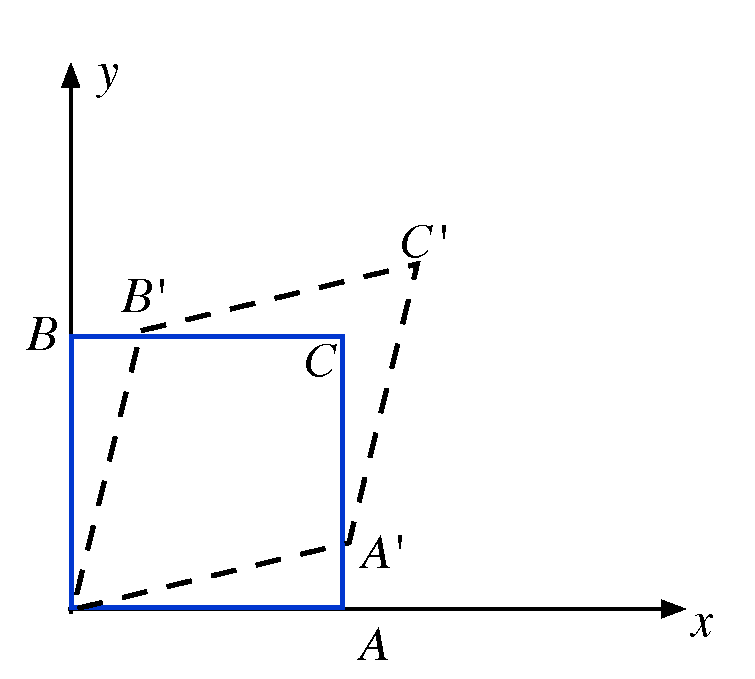
\includegraphics[width=2.5 in]{disto2.pdf}
	\caption{Configuraciones original y deformada de un cuadrado unitario debido a la segunda componente distorsional de la componente simétrica del tensor de transformación de desplazamientos.}
	\label{disto2}
\end{figure}

Finalmente, y en aras de la consistencia apliquemos la componente rotacional $\omega$ (ver \cref{parti}) al cuadrado unitario obteniendo como resultado los siguientes vectors de desplazamientos:

\[{{\vec \Delta }_A} =  - \alpha \hat j\]

\[{{\vec \Delta }_B} = \alpha \hat i\]

\[{{\vec \Delta }_C} = \alpha \hat i - \alpha \hat j\]

y el cambio de configuración mostrado en la \cref{rotarota}

\begin{figure}[H]
\centering
	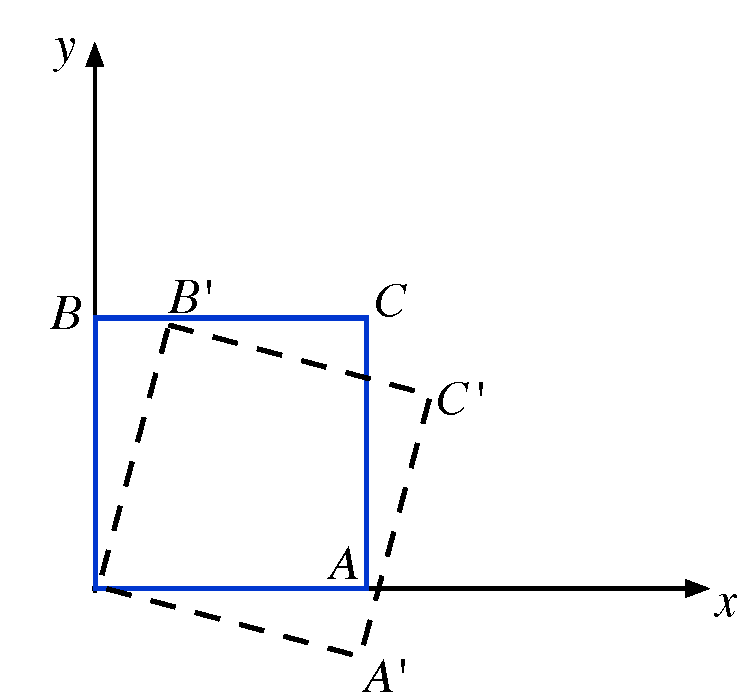
\includegraphics[width=2.5 in]{omega.pdf}
	\caption{Configuraciones original y deformada de un cuadrado unitario debido a la componente anti-simétrica del tensor de transformación de desplazamientos.}
	\label{rotarota}
\end{figure}


\subsection*{Ejemplo}
Un tensor dado $D$ permite calcular los desplazamientos $\Delta$   de los puntos en un espacio (en 2-dimensiones) y cuya posición original se encuentra dada por el vector posición ${\vec r}$   de acuerdo con;

\[\vec \Delta  = D \cdot \vec r\]

El este tensor resulta de superponer (o sumar) los 2 efectos mostrados en la \cref{eje1a} y \cref{eje1b} en la cual las líneas continuas representan la configuración original y las líneas punteadas la configuración final.

\begin{figure}[H]
     \centering
     \subfloat[Cambios debidos a la componente simétrica]{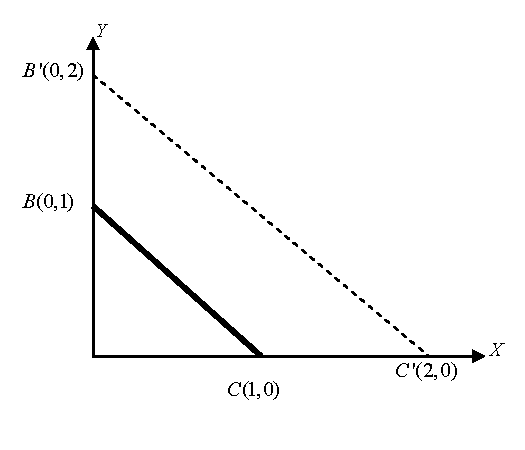
\includegraphics[width=2.8 in]{eje1a.pdf}\label{eje1a}}
     \hspace{0.5cm}
     \subfloat[Cambios debidos a la componente anti-simétrica]{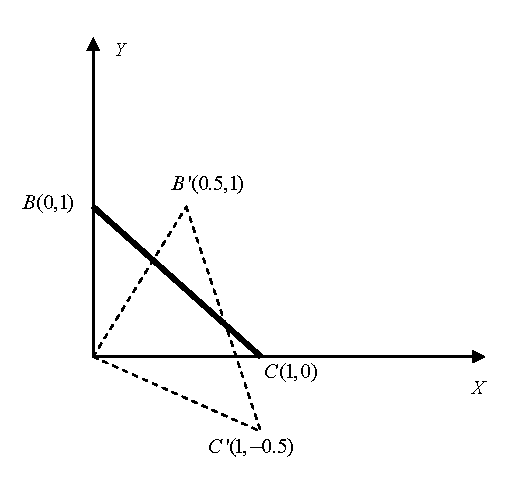
\includegraphics[width=2.8 in]{eje1b.pdf}\label{eje1b}}
     \caption{Transformación líneal de elemento triangular.}
     \label{steady_state1}
\end{figure}

Se pide:

\begin{itemize}
\item (i) Determinar el tensor $D$.
\item (ii) Determinar las componentes simétrica $\varepsilon$ y anti-simétrica $\omega$ del tensor $D$.
\item (iii) Determinar las direcciones y valores principales de la componente simétrica $\varepsilon$.
\end{itemize}

En la primera transformación se tienen los siguientes vectores de posición originales;

\[{\vec r_B} = 1.0\hat j\]
\[{\vec r_C} = 1.0\hat i\]

y los siguientes vectores de desplazamientos para los puntos $B$ y $C$ respectivamente;

\[{\vec \Delta _B} = 1.0\hat j\]
\[{\vec \Delta _C} = 1.0\hat i\]

planteando para cada punto la ecuación:

\[\left\{ {\begin{array}{*{20}{c}}
{{\Delta _x}}\\
{{\Delta _y}}
\end{array}} \right\} = \left[ {\begin{array}{*{20}{c}}
{{\varepsilon _{xx}}}&\bar{\gamma} \\
\bar{\gamma} &{{\varepsilon _{yy}}}
\end{array}} \right]\left\{ {\begin{array}{*{20}{c}}
{{r_x}}\\
{{r_y}}
\end{array}} \right\}\]

permite determinar;

\[\varepsilon \equiv \left[ {\begin{array}{*{20}{c}}
{{\varepsilon _{xx}}}&\bar{\gamma}\\
\bar{\gamma} &{{\varepsilon _{yy}}}
\end{array}} \right] = \left[ {\begin{array}{*{20}{c}}
{1.0}&{0.0}\\
{0.0}&{1.0}
\end{array}} \right].\]

Procediendo de manera análoga en el caso de la segunda transformación se tiene que;

\[\omega  \equiv \left[ {\begin{array}{*{20}{c}}
0&\alpha \\
{ - \alpha }&0
\end{array}} \right] = \left[ {\begin{array}{*{20}{c}}
{0.0}&{0.5}\\
{ - 0.5}&{0.0}
\end{array}} \right]\]

por lo que el tensor resultante corresponde a:

\[\varepsilon  + \omega  \equiv \left[ {\begin{array}{*{20}{c}}
{1.0}&{0.0}\\
{0.0}&{1.0}
\end{array}} \right] + \left[ {\begin{array}{*{20}{c}}
{0.0}&{0.5}\\
{ - 0.5}&{0.0}
\end{array}} \right] \equiv \left[ {\begin{array}{*{20}{c}}
{1.0}&{0.5}\\
{ - 0.5}&{1.0}
\end{array}} \right].\]



\subsection*{Problema propuesto}

La \cref{problem} corresponde a la configuración original de un medio continuo. Si sobre este se aplica el tensor de transformación de desplazamientos:

\[D = \left[ {\begin{array}{*{20}{c}}
{{d_{xx}}}&{{d_{xy}}}\\
{{d_{yx}}}&{{d_{yy}}}
\end{array}} \right]\]


determinar la configuración deformada del medio indicando claramente el efecto de cada una de las componentes definidas de acuerdo con:


\[D = \varepsilon  + \omega  \equiv pI + S + C + \omega \]


\begin{figure}[H]
\centering
	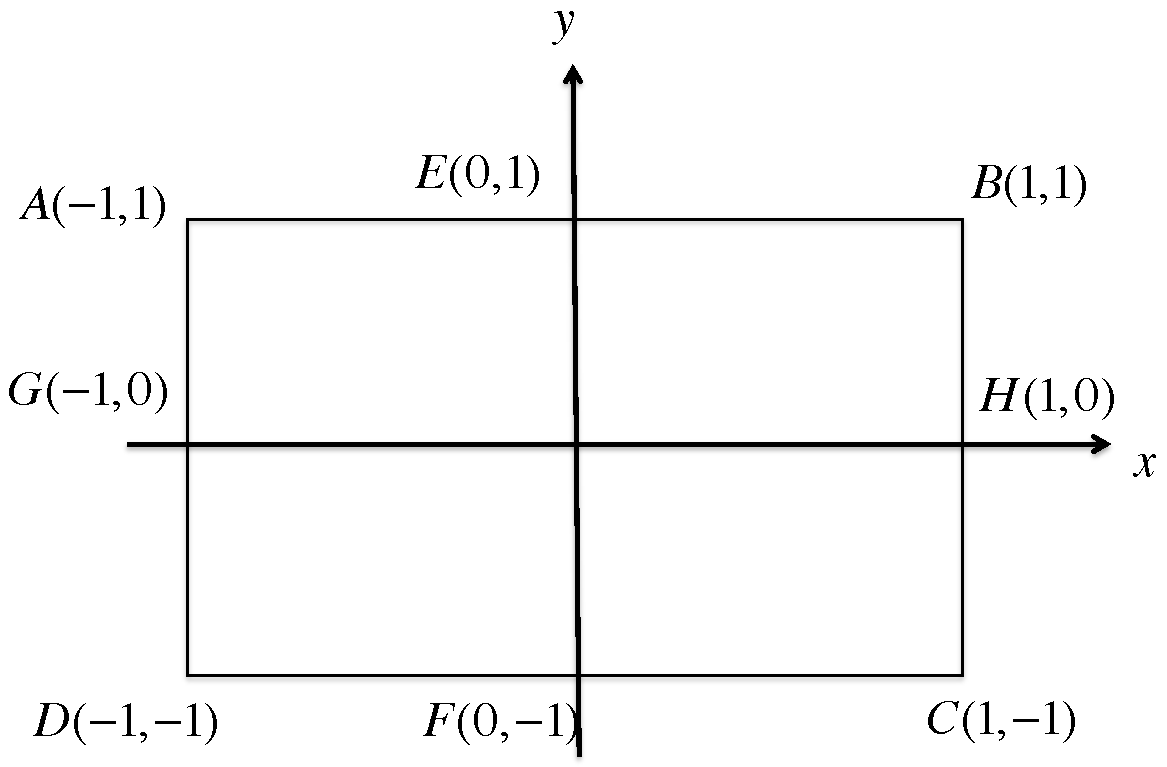
\includegraphics[width=4.0 in]{problemCap5.pdf}
	\caption{Transformación al espacio completo.}
	\label{problem}
\end{figure}


\section{Tensor de deformaciones unitarias}
Procedamos ahora a comparar lo que sucede con una fibra materiales infinitesimal tras haber sido sometida al proceso de deformación. Ésta se muestra en la \cref{pelos} conectando los puntos materiales que ocupan las posiciones $P$ y $Q$ antes de la deformación y las posiciones $p$ y $q$ en la configuración deformada. En la configuración original la fibra $PQ$ esta dada por el vector $d\vec{r}$ expresado en términos de magnitud y dirección como:

\[d\vec r = \hat ndS\]

donde

\[\hat n = \frac{{dx}}{{dS}}\hat i + \frac{{dy}}{{dS}}\hat j.\]

\begin{figure}[H]
\centering
	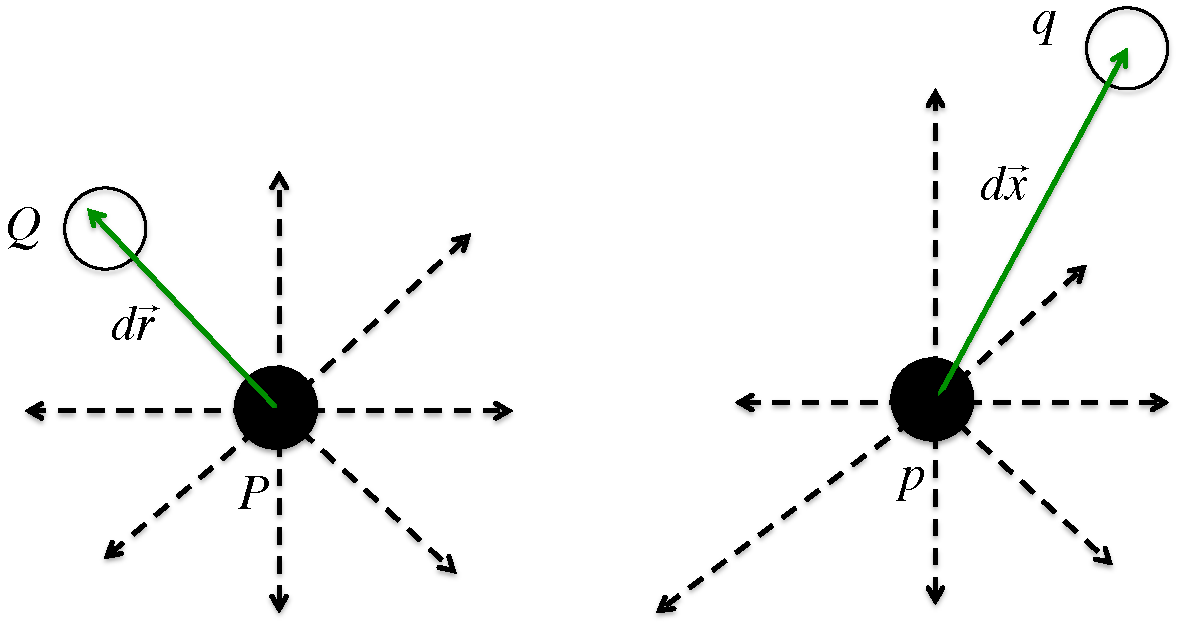
\includegraphics[width=4.0 in]{pelos.pdf}
	\caption{Fibras materiales emanando de un punto material $P$ en las configuraciones original y deformada.}
	\label{pelos}
\end{figure}

En la configuración deformada la fibra $PQ$ se convierte en la fibra $pq$ dada por el vector $d\vec{x}$. Ambas se comparan en la \cref{relative} en la que también se identifica el desplazamiento ${{\vec u}_P}$ del punto material $P$ y el desplazamiento ${{\vec u}_Q}$  del punto material $Q$.

\begin{figure}[H]
\centering
	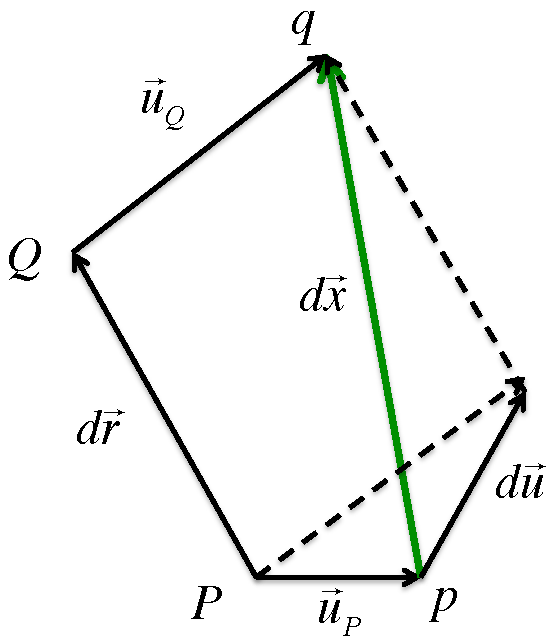
\includegraphics[width=2.5 in]{relative.pdf}
	\caption{Desplazamiento relativo entre 2 puntos materiales infinitesimalmente cercanos.}
	\label{relative}
\end{figure}

Escribiendo el desplazamiento relativo $d\vec u$  en términos de los vectores fibra original y deformado $d\vec{r}$ y $d\vec{x}$  se tiene:

\[d\vec u = d\vec x - d\vec r\]

o usando una relación como:

\[d\vec x = A \cdot d\vec r\]

donde $A$ transforma $d\vec{r}$ en $d\vec{x}$ se tiene:

\[d\vec u = \left[ {A - I} \right] \cdot d\vec r\]

o finalmente:

\begin{equation}
d\vec u = J \cdot d\vec r.
\label{jacobian}
\end{equation}

En la expresión \cref{jacobian} el tensor $J$ \footnote{El tensor $J$ es el análogo al tensor $D$ visto en la sección de trasformaciónes lineales} permite obtener el desplazamiento relativo $d\vec{u}$ del punto material $Q$ con respecto a $P$. Escribiendo $d\vec{u}$ en términos de sus componentes rectangulares como; 

\[d\vec u = du\hat i + dv\hat j\]

permite escribir la \cref{jacobian} en forma explicita de acuerdo con:


\[\left\{ {\begin{array}{*{20}{c}}
{du}\\
{dv}
\end{array}} \right\} = \left[ {\begin{array}{*{20}{c}}
{{J_{xx}}}&{{J_{xy}}}\\
{{J_{yx}}}&{{J_{yy}}}
\end{array}} \right]\left\{ {\begin{array}{*{20}{c}}
{dx}\\
{dy}
\end{array}} \right\}.\]

Reconociendo los términos del tensor $J$ como las variaciones de las componentes rectangulares $du$ y $dv$ a lo largo de distancias diferenciales $dx$ y $dy$ permite escribir:


\[du = {J_{xx}}dx + {J_{xy}}dy \equiv \frac{{\partial u}}{{\partial x}}dx + \frac{{\partial u}}{{\partial y}}dy\]

\[dv = {J_{yx}}dx + {J_{yy}}dy \equiv \frac{{\partial v}}{{\partial x}}dx + \frac{{\partial v}}{{\partial y}}dy\]

o en forma explicita:

\[\left\{ {\begin{array}{*{20}{c}}
{du}\\
{dv}
\end{array}} \right\} = \left[ {\begin{array}{*{20}{c}}
{\frac{{\partial u}}{{\partial x}}}&{\frac{{\partial u}}{{\partial y}}}\\\\
{\frac{{\partial v}}{{\partial x}}}&{\frac{{\partial v}}{{\partial y}}}
\end{array}} \right]\left\{ {\begin{array}{*{20}{c}}
{dx}\\
{dy}
\end{array}} \right\}\]

y en donde el tensor $J$ corresponde al gradiente de desplazamientos. Normalizando el vector de desplazamientos relativos por la magnitud original $dS$ de la fibra, permite obtener el desplazamiento relativo unitario como una transformación

\[\left\{ {\begin{array}{*{20}{c}}
{\frac{{du}}{{dS}}}\\\\
{\frac{{dv}}{{dS}}}
\end{array}} \right\} = \left[ {\begin{array}{*{20}{c}}
{\frac{{\partial u}}{{\partial x}}}&{\frac{{\partial u}}{{\partial y}}}\\\\
{\frac{{\partial v}}{{\partial x}}}&{\frac{{\partial v}}{{\partial y}}}
\end{array}} \right]\left\{ {\begin{array}{*{20}{c}}
{\frac{{dx}}{{dS}}}\\\\
{\frac{{dy}}{{dS}}}
\end{array}} \right\}\]

o

\begin{equation}
\left\{ {\frac{{d\vec u}}{{dS}}} \right\} = J \cdot \hat n.
\label{trans}
\end{equation}

Para identificar los diferentes efectos contenidos en el gradiente de desplazamientos este se descompone en términos de sus componentes simétrica y anti-simétrica como:


\[J = \varepsilon  + \omega \]

o en forma explicita:

\[\left[ {\begin{array}{*{20}{c}}
{\frac{{\partial u}}{{\partial x}}}&{\frac{{\partial u}}{{\partial y}}}\\\\
{\frac{{\partial v}}{{\partial x}}}&{\frac{{\partial v}}{{\partial y}}}
\end{array}} \right] = \left[ {\begin{array}{*{20}{c}}
{\frac{{\partial u}}{{\partial x}}}&{\frac{1}{2}\left( {\frac{{\partial u}}{{\partial y}} + \frac{{\partial v}}{{\partial x}}} \right)}\\\\
{\frac{1}{2}\left( {\frac{{\partial u}}{{\partial y}} + \frac{{\partial v}}{{\partial x}}} \right)}&{\frac{{\partial v}}{{\partial y}}}
\end{array}} \right] + \left[ {\begin{array}{*{20}{c}}
0&{\frac{1}{2}\left( {\frac{{\partial u}}{{\partial y}} - \frac{{\partial v}}{{\partial x}}} \right)}\\\\
{ - \frac{1}{2}\left( {\frac{{\partial u}}{{\partial y}} - \frac{{\partial v}}{{\partial x}}} \right)}&0
\end{array}} \right]\]


Los efectos físicos de las diferentes componentes del tensor $J$ serán estudiados analizando los cambios impuestos por este sobre el elemento diferencial mostrado en la \cref{diferencial}. En particular, se calcularán los desplazamientos de los puntos $A$, $B$ y $C$ con vectores posición:

\[{\vec r_A} = dx\hat i\]
\[{\vec r_B} = dy\hat j\]
\[{\vec r_C} = dy\hat i + dx\hat j. \]


\begin{figure}[H]
\centering
	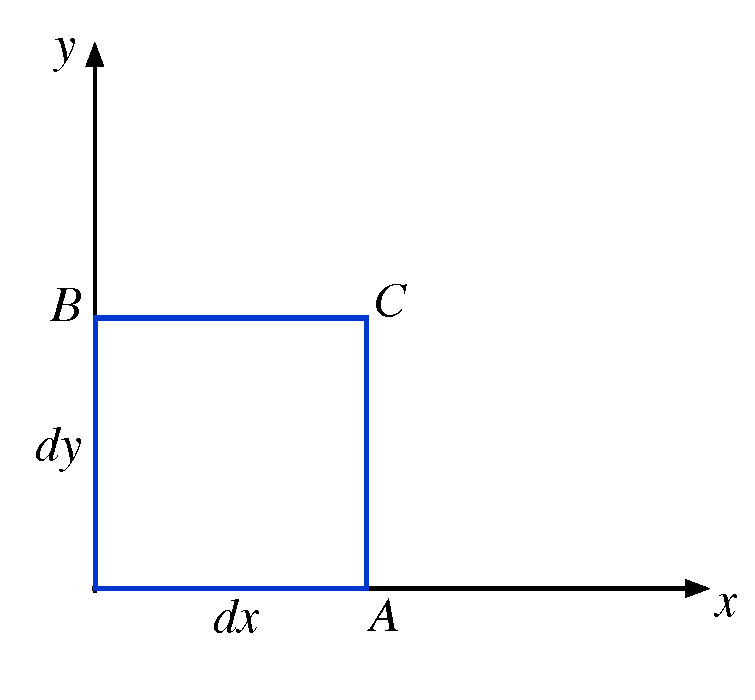
\includegraphics[width=2.5 in]{diferencial.pdf}
	\caption{Elemento diferencial de tamaño $dx \times dy$.}
	\label{diferencial}
\end{figure}


\subsection{Rotación de cuerpo rígido}
Estudiando inicialmente la componente anti-simétrica $\omega$ del tensor $J$ aplicando la transformación sobre el elemento diferencial se tiene respectivamente para los desplazamientos relativos de los puntos $A$, $B$ y $C$:

\[{\left\{ {\begin{array}{*{20}{c}}
{du}\\\\
{dv}
\end{array}} \right\}_A} = \left[ {\begin{array}{*{20}{c}}
0&{\frac{1}{2}\left( {\frac{{\partial u}}{{\partial y}} - \frac{{\partial v}}{{\partial x}}} \right)}\\\\
{ - \frac{1}{2}\left( {\frac{{\partial u}}{{\partial y}} - \frac{{\partial v}}{{\partial x}}} \right)}&0
\end{array}} \right]\left\{ {\begin{array}{*{20}{c}}
{dx}\\
0
\end{array}} \right\} \equiv \left\{ {\begin{array}{*{20}{c}}
0\\
{ - \frac{1}{2}\left( {\frac{{\partial u}}{{\partial y}} - \frac{{\partial v}}{{\partial x}}} \right)dx}
\end{array}} \right\}\]

\[{\left\{ {\begin{array}{*{20}{c}}
{du}\\\\
{dv}
\end{array}} \right\}_B} = \left\{ {\begin{array}{*{20}{c}}
{\frac{1}{2}\left( {\frac{{\partial u}}{{\partial y}} - \frac{{\partial v}}{{\partial x}}} \right)dy}\\\\
0
\end{array}} \right\}\]

\[{\left\{ {\begin{array}{*{20}{c}}
{du}\\\\
{dv}
\end{array}} \right\}_C} = \left\{ {\begin{array}{*{20}{c}}
{\frac{1}{2}\left( {\frac{{\partial u}}{{\partial y}} - \frac{{\partial v}}{{\partial x}}} \right)dy}\\\\
{ - \frac{1}{2}\left( {\frac{{\partial u}}{{\partial y}} - \frac{{\partial v}}{{\partial x}}} \right)dx}
\end{array}} \right\}\]

dando como resultado la configuración deformada de la \cref{crigido}. Rigurosamente, el elemento experimenta un pequeño cambio de volumen (área) considerado como de segundo orden. Claramente esta componente no involucra fuerzas internas o tensiones. De otro lado se debe identificar que la rotación del elemento esta dada por:

\[\omega = \frac{1}{2}\left( {\frac{{\partial u}}{{\partial y}} - \frac{{\partial v}}{{\partial x}}}\right)\]

\begin{figure}[H]
\centering
	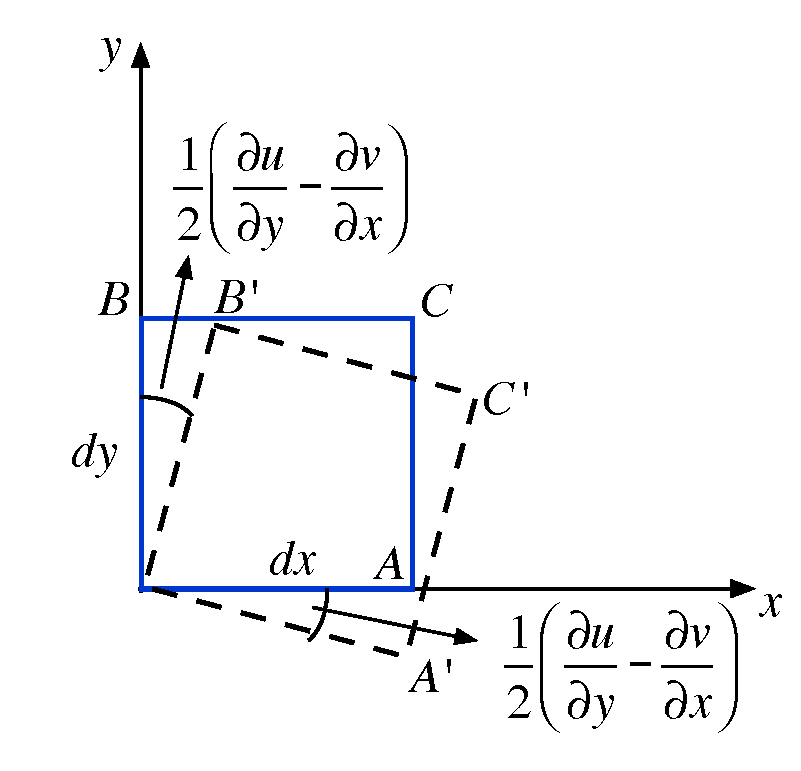
\includegraphics[width=4.0 in]{crigido.pdf}
	\caption{Rotación de cuerpo rígido de un elemento diferencial.}
	\label{crigido}
\end{figure}

\subsection{Componente simétrica $\varepsilon$}
Para el punto A
\[{\left\{ {\begin{array}{*{20}{c}}
{du}\\\\
{dv}
\end{array}} \right\}_A} = \left[ {\begin{array}{*{20}{c}}
{\frac{{\partial u}}{{\partial x}}}&{\frac{1}{2}\left( {\frac{{\partial u}}{{\partial y}} + \frac{{\partial v}}{{\partial x}}} \right)}\\\\
{\frac{1}{2}\left( {\frac{{\partial u}}{{\partial y}} + \frac{{\partial v}}{{\partial x}}} \right)}&{\frac{{\partial v}}{{\partial y}}}
\end{array}} \right]\left\{ {\begin{array}{*{20}{c}}
{dx}\\\\
0
\end{array}} \right\} \equiv \left\{ {\begin{array}{*{20}{c}}
{\frac{{\partial u}}{{\partial x}}dx}\\\\
{\frac{1}{2}\left( {\frac{{\partial u}}{{\partial y}} + \frac{{\partial v}}{{\partial x}}} \right)dy}
\end{array}} \right\}\]

Similarmente para los puntos $B$ y $C$;

\[{\left\{ {\begin{array}{*{20}{c}}
{du}\\\\
{dv}
\end{array}} \right\}_B} = \left\{ {\begin{array}{*{20}{c}}
{\frac{1}{2}\left( {\frac{{\partial u}}{{\partial y}} + \frac{{\partial v}}{{\partial x}}} \right)dy}\\\\
{\frac{{\partial v}}{{\partial y}}dy}
\end{array}} \right\}\]

\[{\left\{ {\begin{array}{*{20}{c}}
{du}\\\\
{dv}
\end{array}} \right\}_C} = \left\{ {\begin{array}{*{20}{c}}
{\frac{{\partial u}}{{\partial x}}dx + \frac{1}{2}\left( {\frac{{\partial u}}{{\partial y}} + \frac{{\partial v}}{{\partial x}}} \right)dy}\\\\
{\frac{1}{2}\left( {\frac{{\partial u}}{{\partial y}} + \frac{{\partial v}}{{\partial x}}} \right)dx + \frac{{\partial v}}{{\partial y}}dy}
\end{array}} \right\}\]

resultando en la configuración mostrada en la \cref{strain}.


\begin{figure}[H]
\centering
	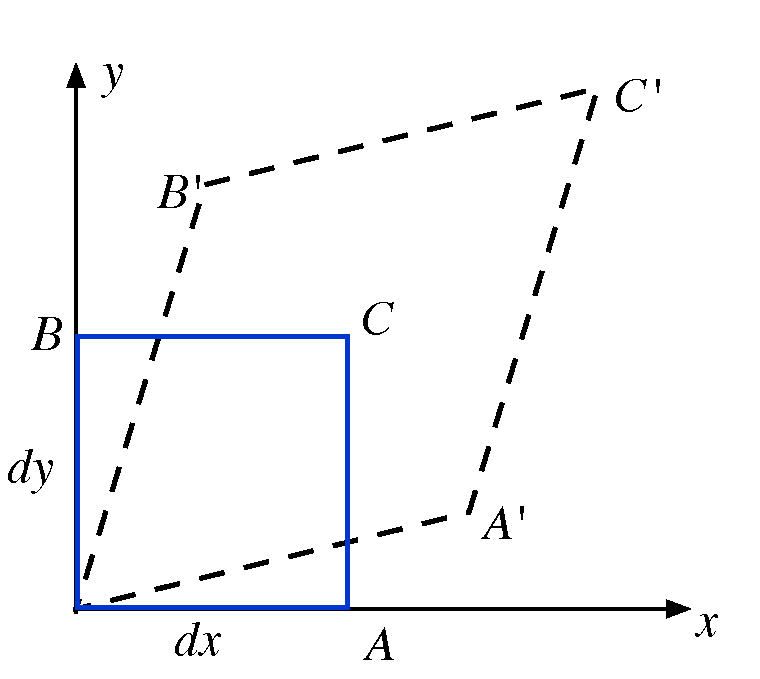
\includegraphics[width=2.5 in]{strain.pdf}
	\caption{Cambio de forma en el elemento diferencial debido a la componente simétrica del gradiente de desplazamientos.}
	\label{strain}
\end{figure}

Ahora estudiemos de manera individual los efectos de los distintos compenentes del tensor simétrico $\varepsilon$.
\subsection{Componente escalar, volumétrica o isotrópica}

\[{\left\{ {\begin{array}{*{20}{c}}
{du}\\\\
{dv}
\end{array}} \right\}_A} = \left[ {\begin{array}{*{20}{c}}
{\frac{1}{2}\left( {\frac{{\partial u}}{{\partial x}} + \frac{{\partial v}}{{\partial y}}} \right)}&0\\\\
0&{\frac{1}{2}\left( {\frac{{\partial u}}{{\partial x}} + \frac{{\partial v}}{{\partial y}}} \right)}
\end{array}} \right]\left\{ {\begin{array}{*{20}{c}}
{dx}\\\\
0
\end{array}} \right\} \equiv \left\{ {\begin{array}{*{20}{c}}
{\frac{1}{2}\left( {\frac{{\partial u}}{{\partial x}} + \frac{{\partial v}}{{\partial y}}} \right)dx}\\\\
0
\end{array}} \right\}\]

\[{\left\{ {\begin{array}{*{20}{c}}
{du}\\\\
{dv}
\end{array}} \right\}_B} = \left\{ {\begin{array}{*{20}{c}}
0\\\\
{\frac{1}{2}\left( {\frac{{\partial u}}{{\partial x}} + \frac{{\partial v}}{{\partial y}}} \right)dy}
\end{array}} \right\}\]

\[{\left\{ {\begin{array}{*{20}{c}}
{du}\\\\
{dv}
\end{array}} \right\}_C} = \left\{ {\begin{array}{*{20}{c}}
{\frac{1}{2}\left( {\frac{{\partial u}}{{\partial x}} + \frac{{\partial v}}{{\partial y}}} \right)dx}\\\\
{\frac{1}{2}\left( {\frac{{\partial u}}{{\partial x}} + \frac{{\partial v}}{{\partial y}}} \right)dy}
\end{array}} \right\}\]



\begin{figure}[H]
\centering
	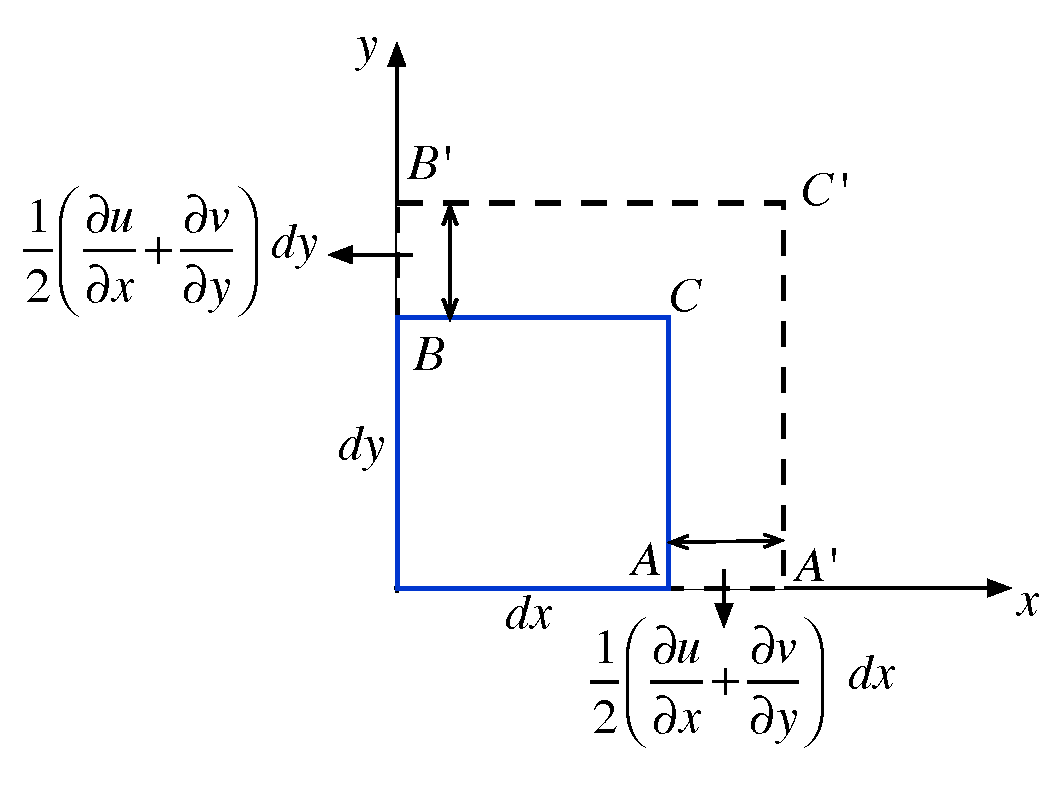
\includegraphics[width=4.0 in]{scalar.pdf}
	\caption{Cambio de forma en el elemento diferencial debido a la componente escalar del gradiente de desplazamientos.}
	\label{scalar}
\end{figure}

\subsection{Componente distorsional}

\[{\left\{ {\begin{array}{*{20}{c}}
{du}\\\\
{dv}
\end{array}} \right\}_A} = \left[ {\begin{array}{*{20}{c}}
{\frac{1}{2}\left( {\frac{{\partial u}}{{\partial x}} - \frac{{\partial v}}{{\partial y}}} \right)}&0\\\\
0&{ - \frac{1}{2}\left( {\frac{{\partial u}}{{\partial x}} - \frac{{\partial v}}{{\partial y}}} \right)}
\end{array}} \right]\left\{ {\begin{array}{*{20}{c}}
{dx}\\\\
0
\end{array}} \right\} \equiv \left\{ {\begin{array}{*{20}{c}}
{\frac{1}{2}\left( {\frac{{\partial u}}{{\partial x}} - \frac{{\partial v}}{{\partial y}}} \right)dx}\\\\
0
\end{array}} \right\}\]

\[{\left\{ {\begin{array}{*{20}{c}}
{du}\\\\
{dv}
\end{array}} \right\}_B} = \left\{ {\begin{array}{*{20}{c}}
0\\\\
{ - \frac{1}{2}\left( {\frac{{\partial u}}{{\partial x}} - \frac{{\partial v}}{{\partial y}}} \right)dy}
\end{array}} \right\}\]

\[{\left\{ {\begin{array}{*{20}{c}}
{du}\\\\
{dv}
\end{array}} \right\}_C} = \left\{ {\begin{array}{*{20}{c}}
{\frac{1}{2}\left( {\frac{{\partial u}}{{\partial x}} - \frac{{\partial v}}{{\partial y}}} \right)dx}\\\\
{ - \frac{1}{2}\left( {\frac{{\partial u}}{{\partial x}} - \frac{{\partial v}}{{\partial y}}} \right)dy}
\end{array}} \right\}\]



\begin{figure}[H]
\centering
	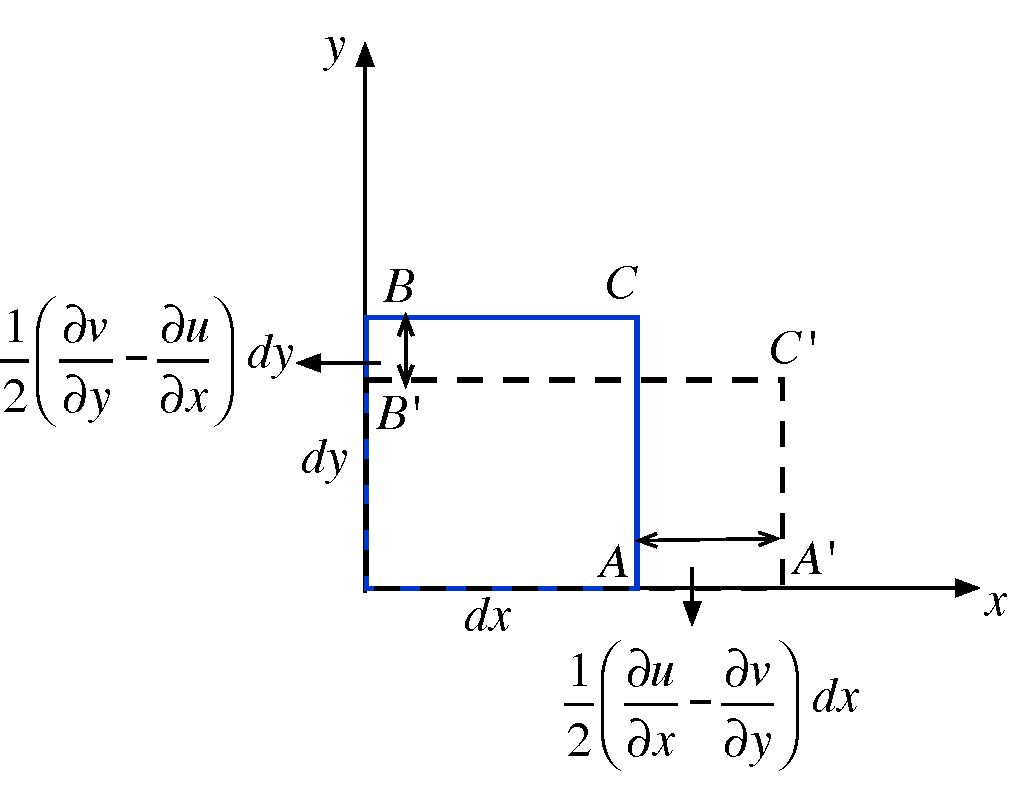
\includegraphics[width=4.0 in]{1dist.pdf}
	\caption{Cambio de forma en el elemento diferencial debido a la primera componente distorsional del tensor de deformaciones unitarias.}
	\label{1dist}
\end{figure}

\[{\left\{ {\begin{array}{*{20}{c}}
{du}\\\\
{dv}
\end{array}} \right\}_A} = \left[ {\begin{array}{*{20}{c}}
0&{\frac{1}{2}\left( {\frac{{\partial u}}{{\partial y}} + \frac{{\partial v}}{{\partial x}}} \right)}\\\\
{\frac{1}{2}\left( {\frac{{\partial u}}{{\partial y}} + \frac{{\partial v}}{{\partial x}}} \right)}&0
\end{array}} \right]\left\{ {\begin{array}{*{20}{c}}
{dx}\\\\
0
\end{array}} \right\} \equiv \left\{ {\begin{array}{*{20}{c}}
0\\
{\frac{1}{2}\left( {\frac{{\partial u}}{{\partial y}} + \frac{{\partial v}}{{\partial x}}} \right)dx}
\end{array}} \right\}\]

\[{\left\{ {\begin{array}{*{20}{c}}
{du}\\\\
{dv}
\end{array}} \right\}_B} = \left\{ {\begin{array}{*{20}{c}}
{\frac{1}{2}\left( {\frac{{\partial u}}{{\partial y}} + \frac{{\partial v}}{{\partial x}}} \right)dy}\\\\
0
\end{array}} \right\}\]

\[{\left\{ {\begin{array}{*{20}{c}}
{du}\\\\
{dv}
\end{array}} \right\}_C} = \left\{ {\begin{array}{*{20}{c}}
{\frac{1}{2}\left( {\frac{{\partial u}}{{\partial y}} + \frac{{\partial v}}{{\partial x}}} \right)dy}\\\\
{\frac{1}{2}\left( {\frac{{\partial u}}{{\partial y}} + \frac{{\partial v}}{{\partial x}}} \right)dx}
\end{array}} \right\}\]

\begin{figure}[H]
\centering
	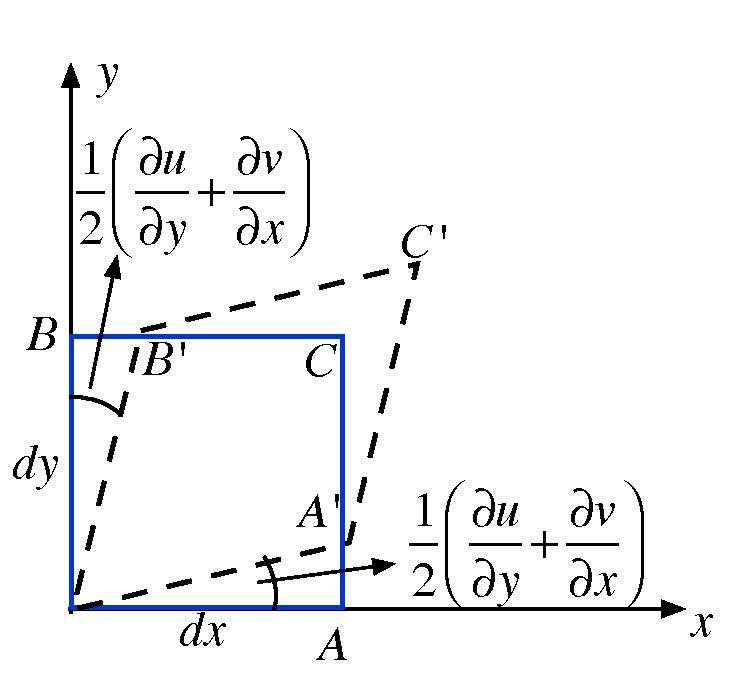
\includegraphics[width=3.0 in]{2dist.pdf}
	\caption{Cambio de forma en el elemento diferencial debido a la segunda componente distorsional del tensor de deformaciones unitarias.}
	\label{2dist}
\end{figure}

Ahora, en el argot ingenieril es común a cada término de la componente simétrica del tensor gradiente de desplazamientos asigarle una nomenclatura particular. Para generalizar la definición consideremos el tensor $\varepsilon$ expresado en coordenasas cartesianas. 
\[	
[\varepsilon] =
\begin{bmatrix}
	\dfrac{\partial u}{\partial x} & \dfrac{1}{2} \left(\dfrac{\partial u}{\partial y} + \dfrac{\partial v}{\partial x}\right)  & \dfrac{1}{2} \left(\dfrac{\partial u}{\partial z} + \dfrac{\partial w}{\partial x}\right) \\\\
	\dfrac{1}{2} \left( \dfrac{\partial v}{\partial x} + \dfrac{\partial u}{\partial y} \right)  & \dfrac{\partial v}{\partial y} & \dfrac{1}{2} \left(\dfrac{\partial v}{\partial z}+\dfrac{\partial w}{\partial y}\right) \\\\
	 \dfrac{1}{2} \left(\dfrac{\partial w}{\partial x} + \dfrac{\partial u}{\partial z} \right) & \dfrac{1}{2} \left(\dfrac{\partial w}{\partial y} + \dfrac{\partial v}{\partial z}\right)  & \dfrac{\partial w}{\partial z}
\end{bmatrix}\]\\

o escrito de otra forma: 
\[	
[\varepsilon] =
\begin{bmatrix}
	\varepsilon_{xx} & \dfrac{1}{2} \gamma_{xy} & \dfrac{1}{2} \gamma_{xz}  \\\\
	\dfrac{1}{2} \gamma_{xy}  & \varepsilon_{yy} & \dfrac{1}{2}  \gamma_{yz}  \\\\
	 \dfrac{1}{2} \gamma_{xz} & \dfrac{1}{2} \gamma_{yz}  &  \varepsilon_{zz}
\end{bmatrix}\]\\

En donde $\varepsilon_{xx}$, $\varepsilon_{yy}$ y $\varepsilon_{zz}$ son conocidas como deformaciones axiales o normales y  $\gamma_{xy}$ ,$ \gamma_{xz}$  y $\gamma_{yz}$  como deformaciones angulares o deformaciones por cortante. 

Por otro lado, la componente rotacional podría escribirse 

\[	
[\omega] =
\begin{bmatrix}
	0 & \omega_{xy}  &  \omega_{xz} \\\\
	 -\omega_{xy}  & 0 &  \omega_{yz} \\\\ 
	 -\omega_{xz}  & -\omega_{yz}  &  0
\end{bmatrix}\] 

en donde $\omega_{xy}$, $\omega_{xz}$ y  $\omega_{yz}$ representan la rotación de cuerpo rígido respecto a los ejes $z$, $y$ y $x$ respectivamente. 


Para terminar, el tensor $\varepsilon$ en coordenas cilindricas está definido como:  

\[	
[\varepsilon] =
\begin{bmatrix}
	\varepsilon_{rr} & \dfrac{1}{2} \gamma_{r\theta} & \dfrac{1}{2} \gamma_{rz}  \\\\
	\dfrac{1}{2} \gamma_{r\theta}  & \varepsilon_{{\theta}{\theta}} & \dfrac{1}{2}  \gamma_{{\theta}z}  \\\\
	 \dfrac{1}{2} \gamma_{rz} & \dfrac{1}{2} \gamma_{{\theta}z}  &  \varepsilon_{zz}
\end{bmatrix}\]


\begin{equation*}	
	\varepsilon_{rr} = \dfrac{\partial u}{\partial r}
	\hspace{1cm}
	\varepsilon_{\theta \theta} = \dfrac{u}{r} + \dfrac{1}{r} \dfrac{\partial v}{\partial \theta}
	\hspace{1cm}
	\varepsilon_{zz} = \dfrac{\partial w}{\partial z} 
\end{equation*}

\begin{equation*}	
	\gamma_{r \theta} = \dfrac{1}{r} \dfrac{\partial u}{\partial \theta} + \dfrac{\partial v}{\partial r} - \dfrac{v}{r} 
	\hspace{1cm}
	\gamma_{\theta z} = \dfrac{\partial v}{\partial z} + \dfrac{1}{r} \dfrac{\partial w}{\partial \theta} 
	\hspace{1cm}
	\gamma_{rz}	 = \dfrac{\partial u}{\partial z} + \dfrac{\partial w}{\partial r}
\end{equation*}

\section*{Ejemplo}

El campo de desplazamientos para la cuña auto-soportada mostrada en la \cref{wedge} esta dado por:

\begin{equation*}	
	u = \frac{S}{E}{K_1}\left( {\nu ,\phi } \right)\left( {x - \ell {C_\phi }} \right)
	\hspace{2cm}
	v =  - \frac{S}{E}{K_2}\left( {\nu ,\phi } \right)y
\end{equation*}

donde $u$ y $v$ corresponden a los desplazamientos en las direcciones horizontal y vertical respectivamente y ${K_1}\left( {\nu ,\phi } \right)$ y ${K_2}\left( {\nu ,\phi } \right)$ son constantes que dependen del semi-ángulo de la cuña y del material. $E$ es una constante que depende del material. 
\begin{figure}[H]
\centering
	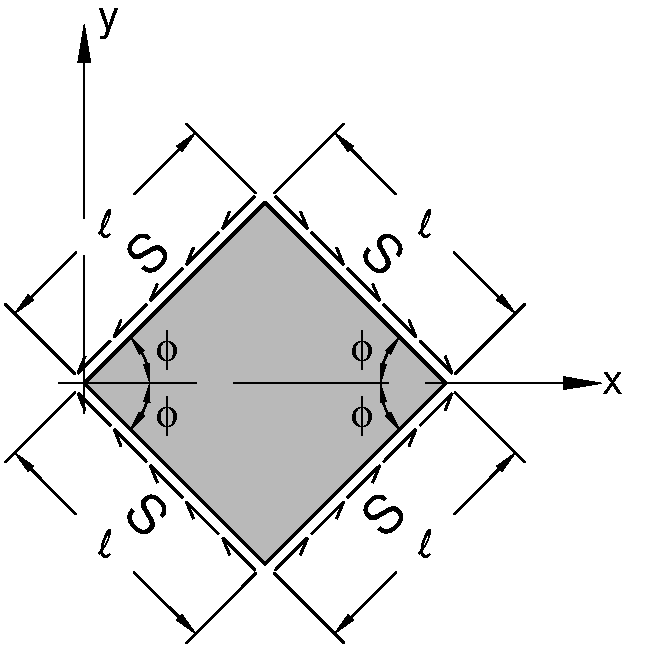
\includegraphics[width=2.8 in]{wedge.pdf}
	\caption{Cuña auto-soportada.}
	\label{wedge}
\end{figure}

\begin{itemize}
\item[•] Esbozar la configuración deformada (final) de la cuña
\item[•] Los tensores gradiente de desplazamientos $J$, deformaciones unitarias $\epsilon$ y rotaciones $\omega$.
\item[•] Determinar las direcciones de máximo cambio de tamaño y máxima rotación.
\end{itemize}

Para esbozar la configuración deformada de la cuña es preciso evaluar el campo de desplazamientos en puntos de la misma. Por la linealidad de las funciones del campo de desplazamientos $u$ y $v$ y por la simetría del problema, en este caso reviremos lo que pasa en cada una de las esquinas \footnote{para funciones de desplazamiento más complejas puede ser preciso usar métodos más elaborados para la evaluación de dichas funciones}. Es decir, evaluamos los desplazamientos en los puntos $A = (0,0)$,  $B = (lcos\phi,l sen\phi)$, $C = (lcos\phi,-lsen\phi)$ y $D = (2lcos\phi,0)$. En la \cref{wedgedef} se muestra esquematicamente en linea punteada la configuración deformada de la cuña. Nótese  como los puntos ubicados en el eje de simetría $A-D$ solo tienen desplazamiento en $x$, $u$, miéntras que los puntos en el eje de simetría $B-C$ solo en $y$, $v$. El punto central del medio continuo no se desplaza. 

\begin{figure}[H]
\centering
	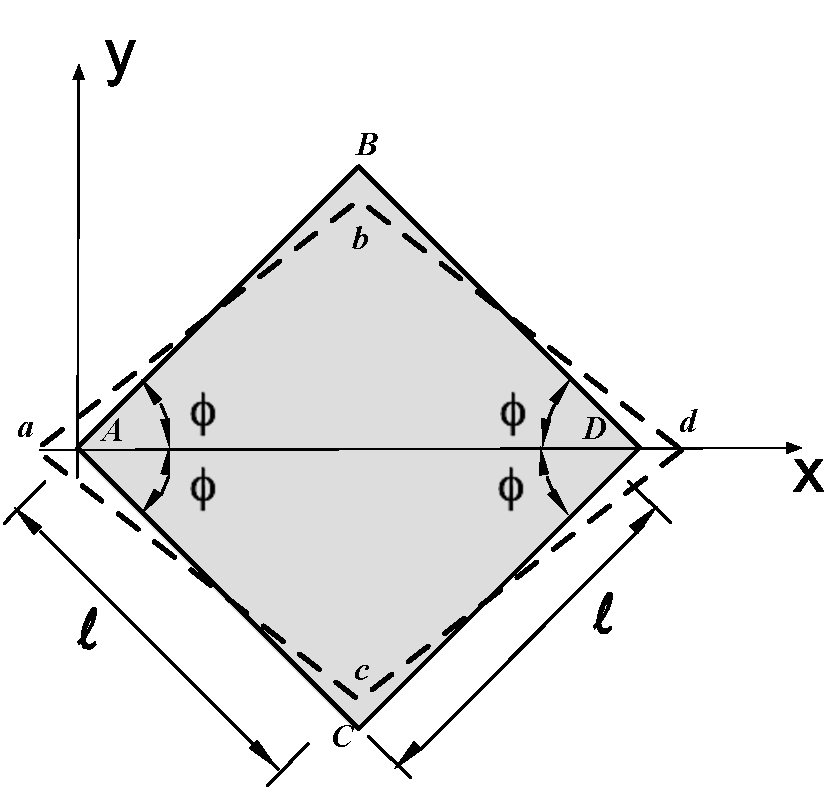
\includegraphics[width=3.0 in]{wedgedef.pdf}
	\caption{Configuación final Cuña auto-soportada.}
	\label{wedgedef}
\end{figure}

Por otro lado, el tensor gradiente de desplazamientos está dado por: 


\[J = \frac{S}{E}\left[ {\begin{array}{*{20}{c}}
{{K_1}\left( {\nu ,\phi } \right)}&0\\
0&{ - {K_2}\left( {\nu ,\phi } \right)}
\end{array}} \right]\]

\[\varepsilon  \equiv J\]

En este caso las rotaciones de cuerpo rígido son nulas

\[\omega  = 0\]

 Nótese que el tensor $\varepsilon $ ya está escrito en sus valores principales, lo que quiere decir que las deformaciones axiales máximas están dadas por: $\frac{S}{E}{K_1}\left( {\nu ,\phi }\right) $ como el estiramiento máximo. y $ \frac{S}{E} {K_2}\ \left({\nu ,\phi } \right)$  como el acortamiento máximo.

\subsection{Ejemplo: Barra apoyada sometida a su peso propio}

%
En la  \cref{BarApo} se muestra un elemento de secci\'on circular de radio $R$, altura $H$, apoyado en su extremo inferior y que est\'a sometido solamente a la acci\'on de su peso propio. Se indica el campo de desplazamientos en el sistema coordenado $xyz$.\\
%
\begin{equation*}	
	u= \nu \dfrac{\gamma}{E} z x 
	\hspace{2cm}
	v= \nu \dfrac{\gamma}{E} z y 
	\hspace{2cm}
	w= -\dfrac{\gamma}{2E} z^2 - \dfrac{\gamma \nu}{2E} (x^2+y^2)+\dfrac{\gamma}{2E} H^2  
\end{equation*}
%
Donde 	$u,v,w$ son los desplazamientos asociados a los ejes $x,y,z$ respectivamente. $E$, $\gamma$ y $\nu$ son constantes del material. \\ 		
\begin{figure}[h]
	\centering
	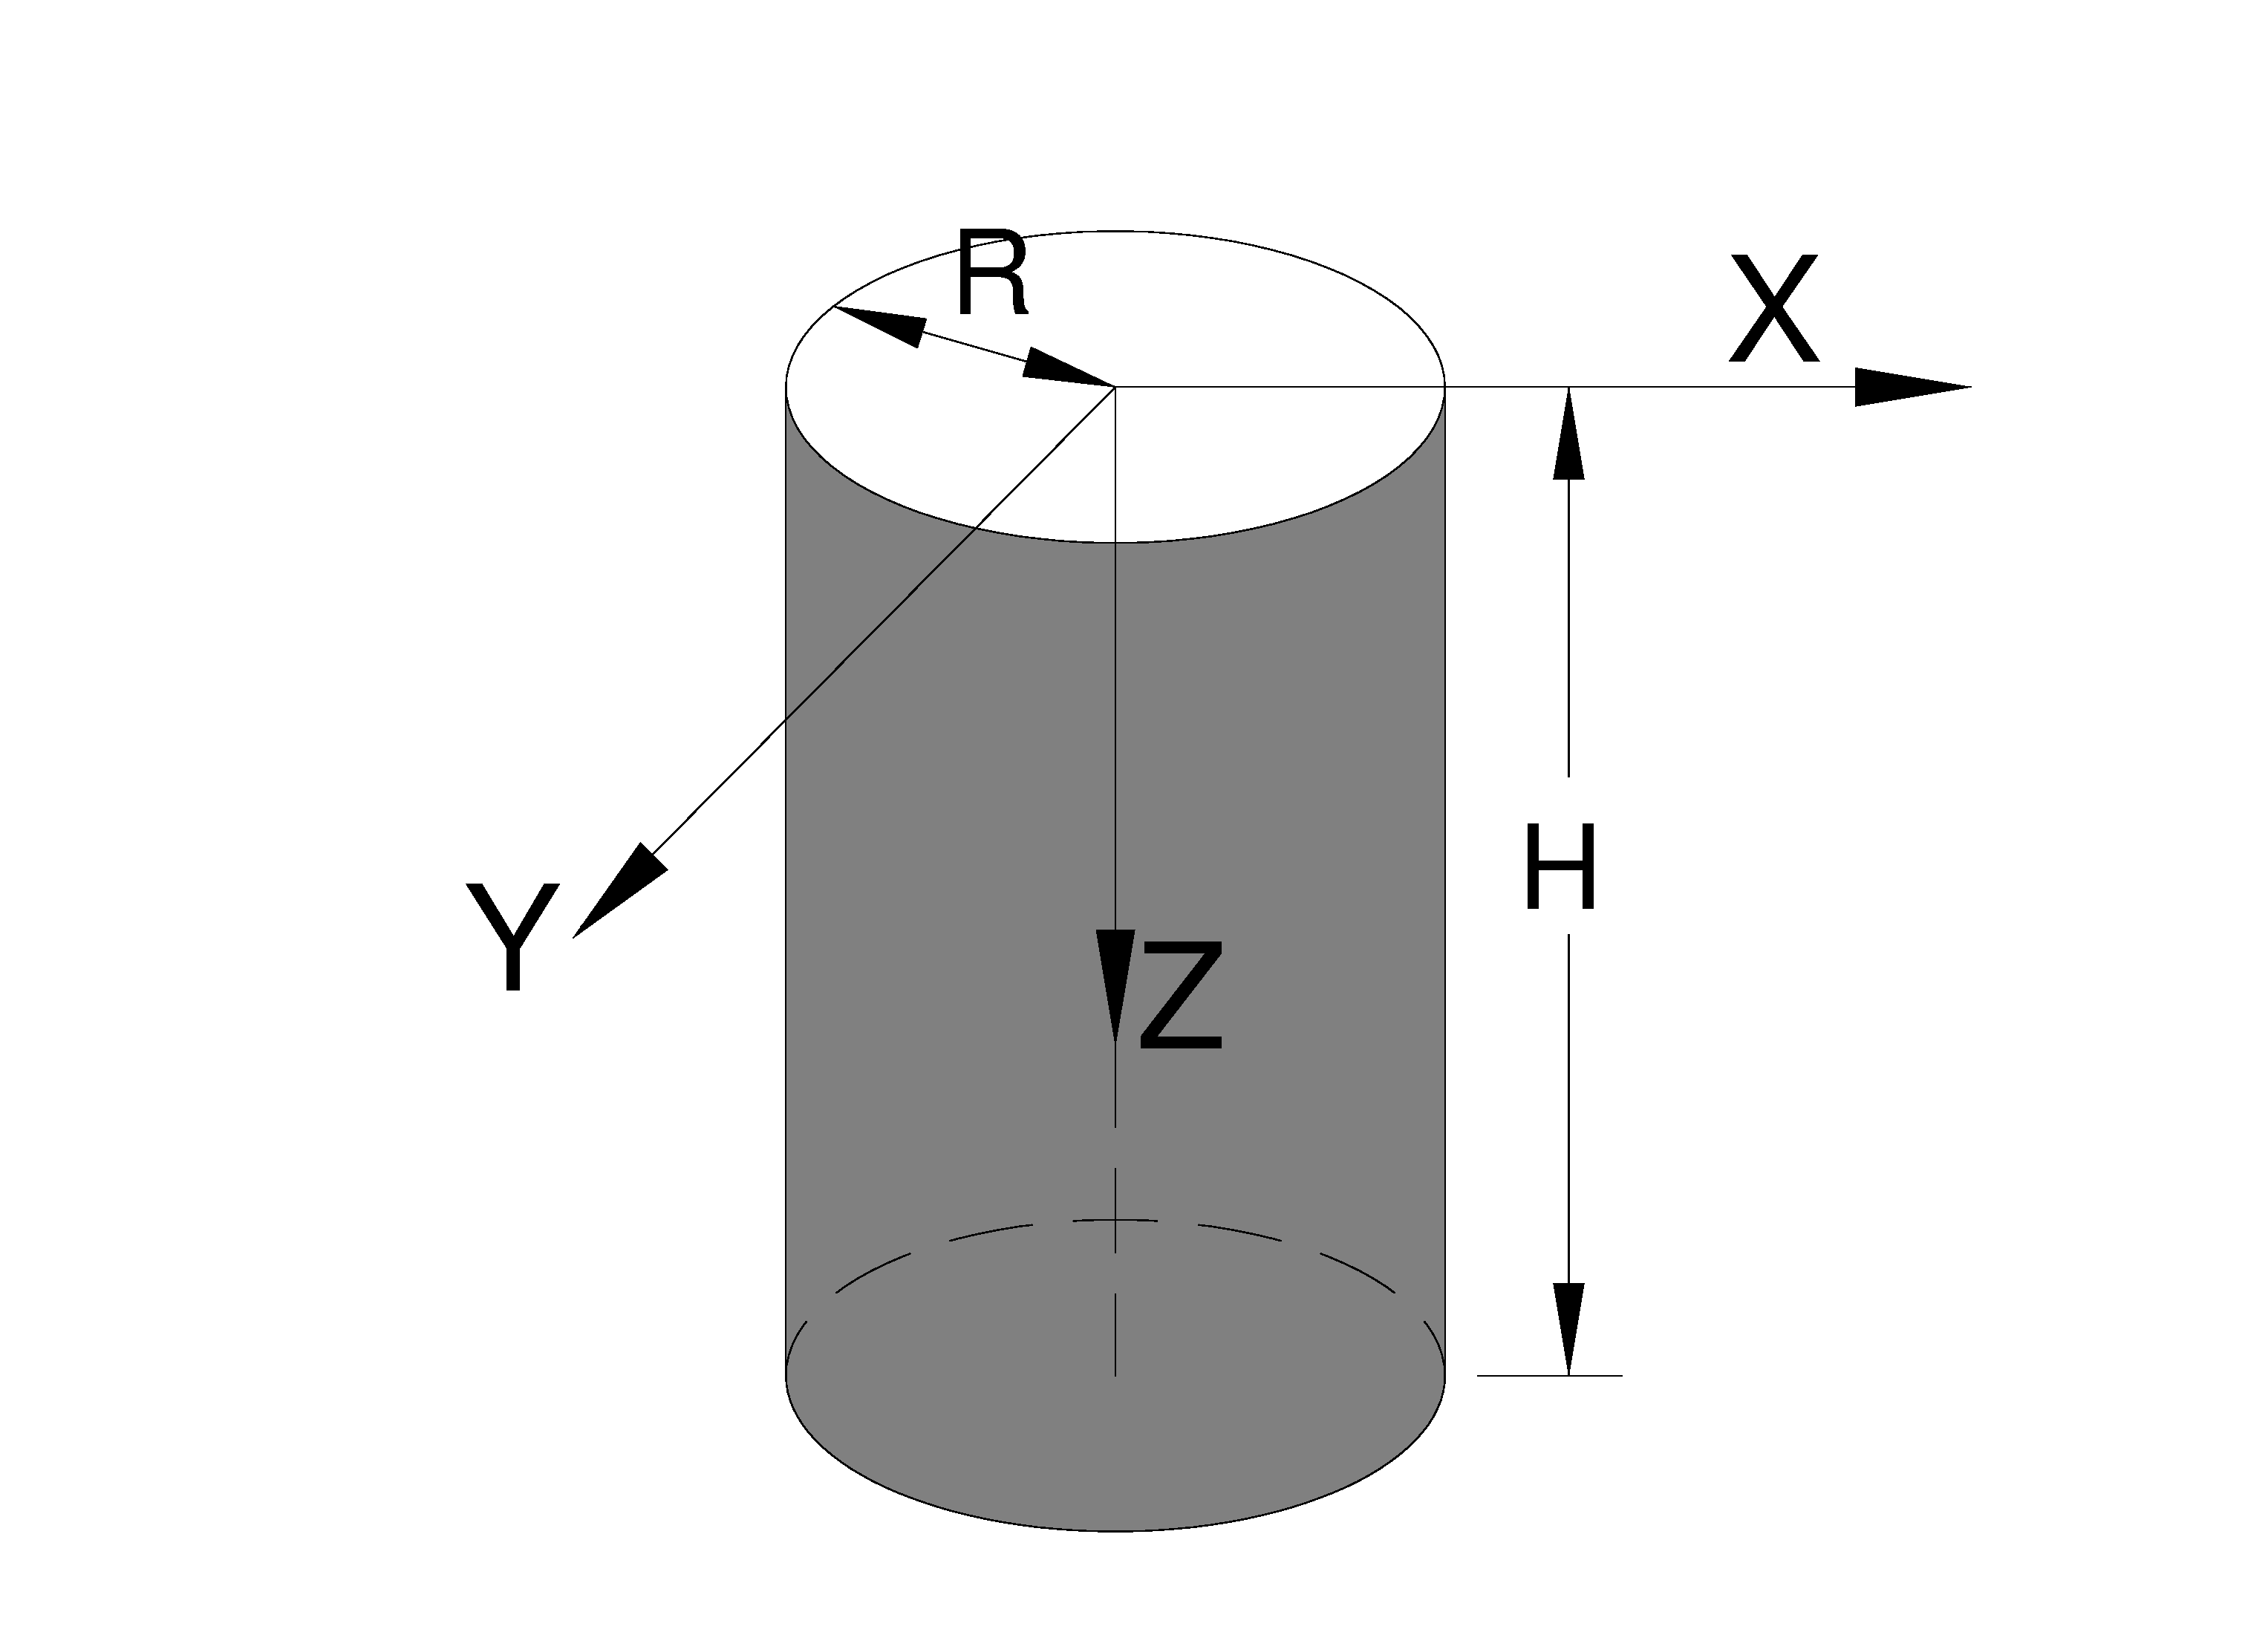
\includegraphics[height=6cm]{barraapoyada.pdf}
	\caption{Barra apoyada}
	 \label{BarApo}
\end{figure}\\
%
\begin{enumerate}
% 
	\item[•] Esboce la configuraci\'on deformada de la barra.\\
	
	\textbf{Solución:}\\
	
	Para esbozar una configuración deformada lo hacemos a partir del campo de desplazamientos $u$, $v$, $w$. Para realizarla  hagamos un corte transversal (plano $xy$) y un corte longitudinal (plano $xz$) y evaluemos que pasa con los desplazamientos en algunos puntos de la frontera. \\
	
$x = 0,  \;\;  y = 0,  \;\; z = 0.  \;\;   \Longrightarrow  \;\; u = 0,  \;\;\;   v = 0, \;\;\;   w = \dfrac{\gamma}{2E} H $\\\\
$x =\pm R,  \;\;  y = 0,  \;\; z = 0.  \;\;   \Longrightarrow  \;\; u = 0,  \;\;\;   v = 0, \;\;\;   w = - \dfrac{\gamma \nu}{2E} R^2 +  \dfrac{\gamma}{2E} H^2$  \\\\
$x =0,  \;\;  y = \pm R,  \;\; z = 0.  \;\;   \Longrightarrow  \;\; u = 0,  \;\;\;   v = 0, \;\;\;   w = - \dfrac{\gamma \nu}{2E} R^2 +  \dfrac{\gamma}{2E} H^2$  \\\\
$x = 0,  \;\;  y = 0,  \;\; z = H.  \;\;   \Longrightarrow  \;\; u = 0,  \;\;\;   v = 0, \;\;\;   w = 0$  \\\\
$x = \pm R,  \;\;  y = 0,  \;\; z = H.  \;\;   \Longrightarrow  \;\; u =\pm \nu \dfrac{\gamma}{E} H R,   \;\;\;   v = 0, \;\;\;   w = - \dfrac{\gamma \nu}{2E} R^2$  \\\\
$x = 0,  \;\;  y = \pm R,  \;\; z = H.  \;\;   \Longrightarrow  \;\; u =0,   \;\;\;   v = \pm \nu \dfrac{\gamma}{E} H R, \;\;\;   w = - \dfrac{\gamma \nu}{2E} R^2$  \\

En la figura \cref{ConDef} aparecen la configuración inicial (línea punteada) y final del elemento. 

\begin{figure}[h]
	\centering
	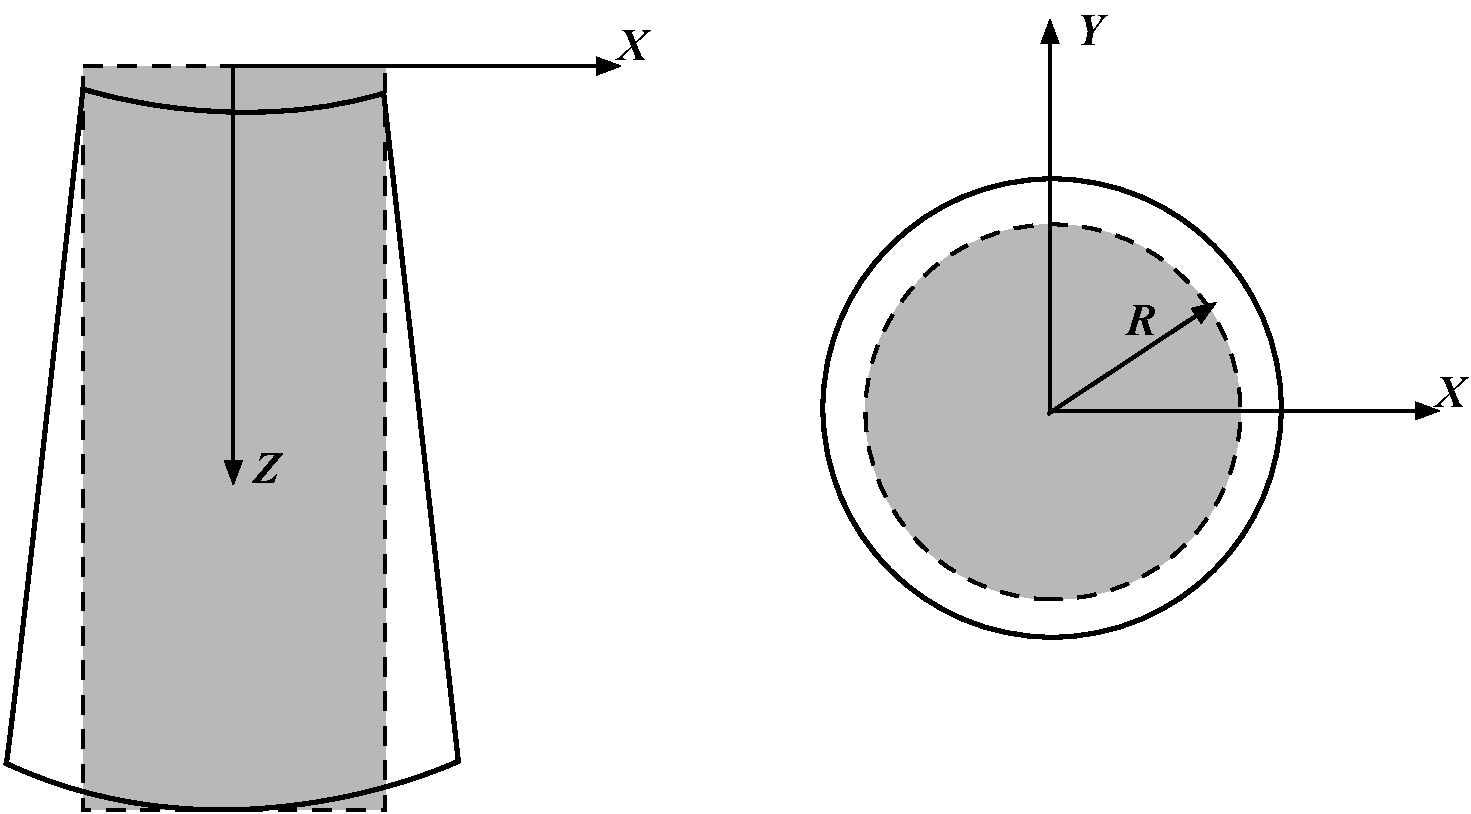
\includegraphics[height=4.5cm]{Configura.pdf}
	\caption{Cortes con configuración final}
	 \label{ConDef}
\end{figure}
%	
	\item[•] Calcule el tensor de deformaciones y descompóngalo en $[\varepsilon]$ (sim\'etrico) y $[\omega]$ (asim\'etrico).
		
	\textbf{Solución:}\\
	
	El tensor gradiente de desplazamientos está dado por: 
	
	\[[D]
 	=   \dfrac{\gamma}{E}
 	\begin{bmatrix}
     	 \nu  z & 0 &  \nu  x\\
     	0 &  \nu  z &  \nu  y\\
     	- \nu x & - \nu  y &  - z\\
 	\end{bmatrix} \]
 	
 	El tensor  $\varepsilon$ y $\omega$ está dado por: 
 		\[[\varepsilon]
 	= \dfrac{\gamma}{E}
 	\begin{bmatrix}
     	 \nu  z & 0 &  0\\
     	0 &  \nu  z &  0\\
     	0 & 0 &  -  z\\
 	\end{bmatrix} 
 	\hspace{2cm}
 	[\omega]
 	= \dfrac{\gamma}{E}
 	\begin{bmatrix}
     	 0 & 0 &  \nu x\\
     	0 & 0 &  \nu y\\
     	- \nu x & - \nu  y &  0\\
 	\end{bmatrix} \]
	%
	\item[•]¿Cuáles son los valores m\'aximos y m\'inimos de las deformaciones axiales y en que puntos se presentan? \\
		
	\textbf{Solución:} \\
	
$\varepsilon_{xx} =  \nu \dfrac{\gamma}{E} z  \;\; \Longrightarrow  \;\; \varepsilon_{min} = 0  \;\;\; (z=0),  \;\;\;\;  \varepsilon_{max} = \nu \dfrac{\gamma}{E} H \;\;\; (z=H) $\\\\
$\varepsilon_{yy} =  \nu \dfrac{\gamma}{E} z  \;\; \Longrightarrow  \;\; \varepsilon_{min} = 0  \;\;\; (z=0),  \;\;\;\;  \varepsilon_{max} = \nu \dfrac{\gamma}{E} H \;\;\; (z=H)$ \\\\
$\varepsilon_{zz} =  - \dfrac{\gamma}{E} z  \;\; \Longrightarrow  \;\; \varepsilon_{min} = 0  \;\;\; (z=0),  \;\;\;\;  \varepsilon_{max} = - \dfrac{\gamma}{E} H \;\;\; (z=H)$ \\
	%
	\item[•] ¿Cuáles son los valores m\'aximos y m\'inimos de los desplazamientos $u$, $v$ y $w$ y en que puntos se presentan?
		

$u =  \nu \dfrac{\gamma}{E} zx  \;\; \Longrightarrow  \;\; u_{min} = 0  \;\;\; (x=0),  \;\;\;\;  u_{max} =\abs{ \nu \dfrac{\gamma}{E} HR} \;\;\; (z=H, x=\abs{R})$ \\\\
$v =  \nu \dfrac{\gamma}{E} zy  \;\; \Longrightarrow  \;\; v_{min} = 0  \;\;\; (y=0),  \;\;\;\;  v_{max} =\abs{ \nu \dfrac{\gamma}{E} HR} \;\;\; (z=H, y=\abs{R})$ \\

	Para el caso del desplazamiento en $z$ los máximos dependen de la relación entre $H^2$ y $R^2=x^2 + y^2$. Supongamos $H>R$. 
	

$w_{min} = 0  \;\;\; ( x=y=0,z=H),  \;\;\;\;  w_{max} = \dfrac{\gamma}{2E} H^2  \;\;\; ( x=y=z=0)$ \\


	%
	\item[•]¿Existen puntos exentos de rotaci\'on de cuerpo r\'igido?, responda s\'i o no y justifique su respuesta.\\
	
	\textbf{Solución:}\\
	
	Sí, si existen puntos exentos de rotación. La línea longitudinal cuando $x=y=0$ no experimenta rotación de cuerpo rígido. 
	 
	\item[•]¿Es posible encontrar puntos sometidos a deformación angular?, responda s\'i o no y justifique su respuesta. \\
	
		\textbf{Solución:}\\
		
		Sí es posible. Como puede verse en el tensor  $\varepsilon$ los valores principales son diferentes, por lo es posible encontrar alguna dirección sometida a deformación angular.
%
\end{enumerate}

\textbf{Tarea}

Describa la configuración deformada de las partículas. 


\section{Ejercicios}


\begin{enumerate}

\item \label{punto01_d} En la  figura \ref{fig1} se muestra la configuración inicial y final en donde las coordenadas puntos son A, B, C y D son A(1,1), B(-1,-1), C($-\sqrt{2}/2,\sqrt{2}/2$), D($\sqrt{2}/2,-\sqrt{2}/2$) . Sabiendo que $\vec{r}$ es el vector de posici\'on original, $\vec{\rho}$ es el vector de posición final y  $\vec{\vartriangle}$ es vector de desplazamiento 

	\begin{enumerate}
	\item Determinar la matriz de desplazamientos lineales $[D]$ tal que	$\vec{\vartriangle}=  D  \centerdot  \vec{r}$. 
	\item Derterminar la matriz de transformaci\'on lineal $[A]$ tal que $\vec{\rho}= A \centerdot \vec{r}$	
	\item Descomponer $[D]$ en componente sim\'etrica y componente asim\'etrica. Mostrar graficamente lo efectos. 	
	\item  Usando el circulo de Mohr, determinar las direcciones principales y los valores propios de la matriz de transformaci\'on lineal sim\'etrica.
	\end{enumerate}
	
	\begin{figure}[H]
		\centering	
	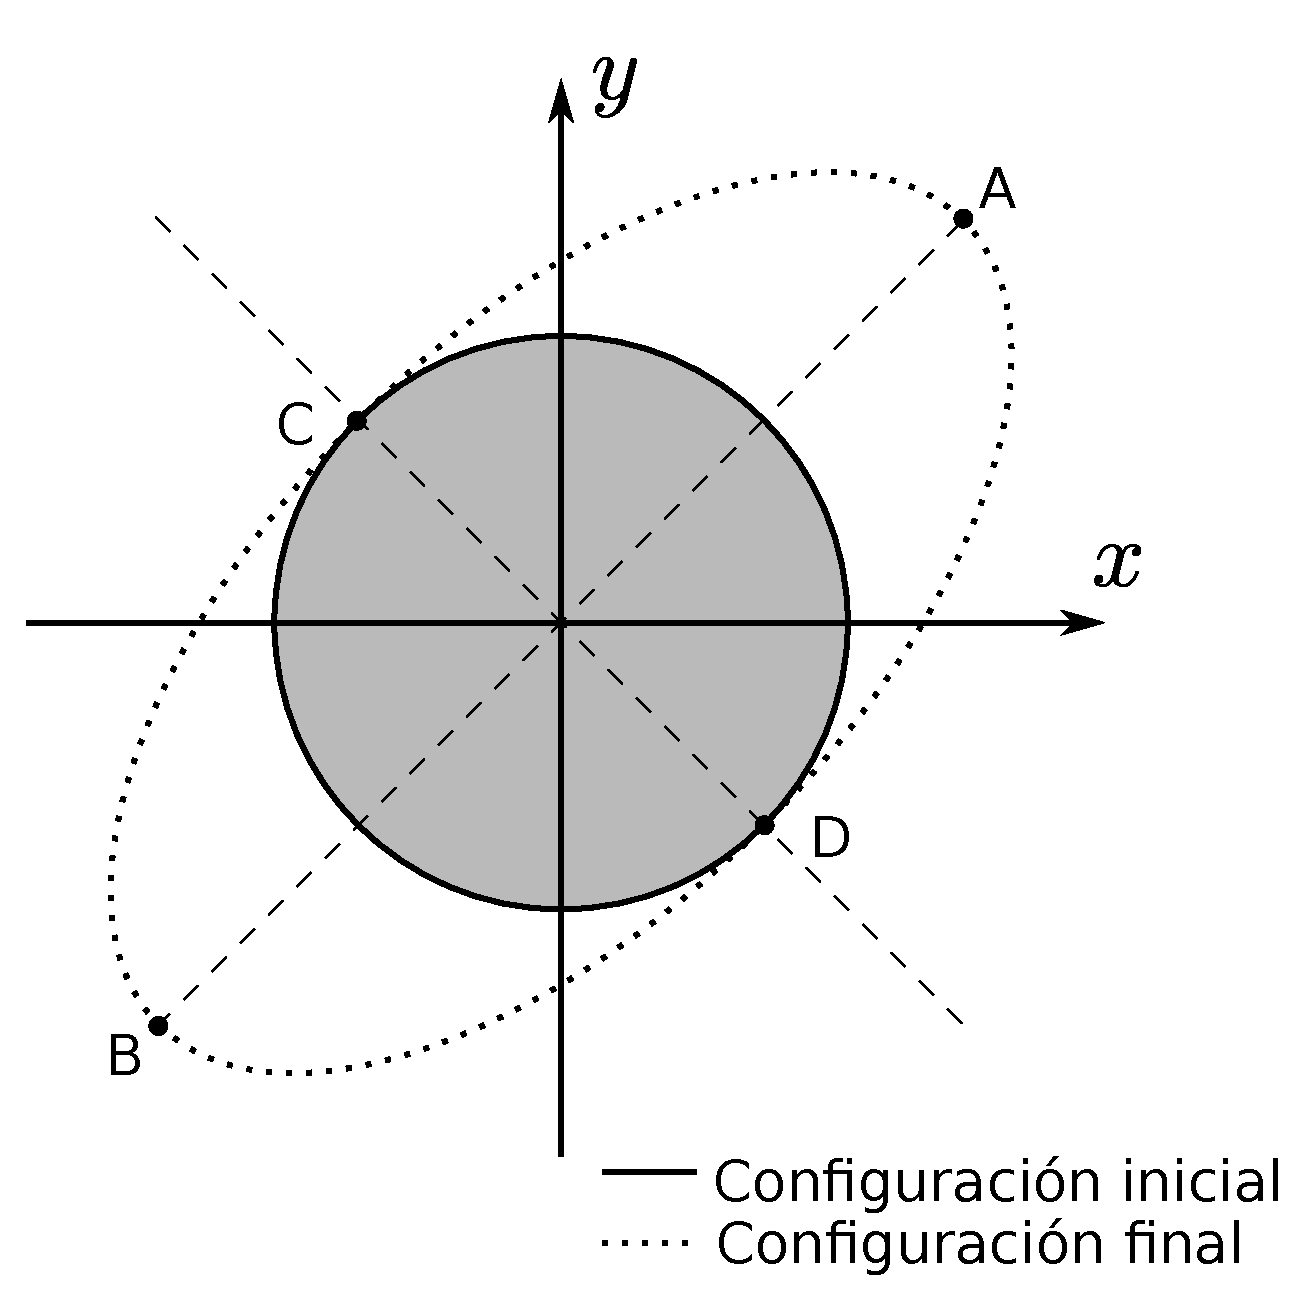
\includegraphics[scale=0.4]{Elipse.pdf}\\
		\caption{Transformaci\'on lineal}
	\label{fig1}
	\end{figure}
	
\newpage

	\item  \label{punto02_d} En la figura \cref{Triangulo} se muestra la configuraci\'on inicial y final (linea punteada) del un triángulo de lado unitario formado por los puntos A, B, C. Para pasar de la configuración inicial a la final se aplica una trasformación lineal de desplazamientos $[D]$, tal que $\lbrace{\Delta}\rbrace = [D]\cdot\lbrace{r}\rbrace$, donde $\Delta$ es el vector desplazamiento, y $r$ es el vector posici\'on inicial.
%
\begin{figure}[H]
	\centering
	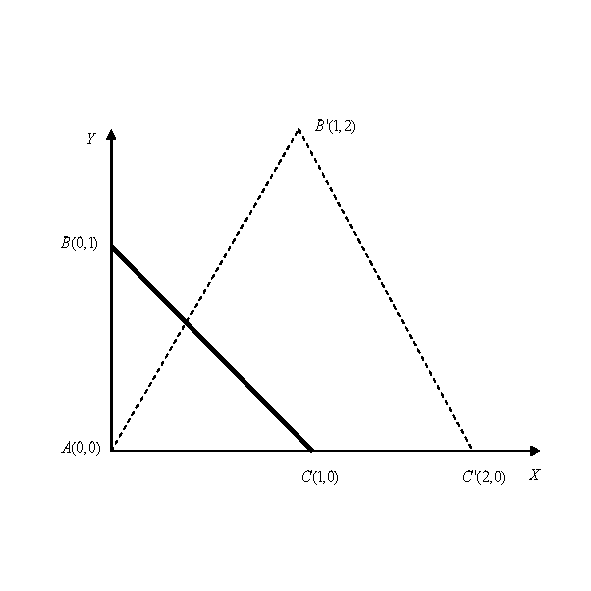
\includegraphics[height=9cm]{Triangulo.pdf} 
	\caption{Configuraciones inicial y deformada}
	\label{Triangulo}
\end{figure}

\begin{enumerate}
\item Determinar la transformación lineal $[D]$, y descomponerla en sus componente simétrica $[\varepsilon]$ y asimétrica $[\omega]$.
\item Determinar las direcciones principales de la transformación $[D]$. Es posible usar circulo de Morh.
\item Mostrar matemática y gráficamente el efecto independiente de las diferentes componentes del tensor lineal de desplazamientos. Las componentes a considerar son la isotrópica, las distorsionales y la rotación de cuerpo rígido, tal que $[D] = p[I] + [S] +[C] + [\omega]$
\item Escribir en sus direcciones principales la componente simétrica $[\varepsilon]$ de la transformación $[D]$.
\end{enumerate}

\newpage
\item  \label{punto03_d} La figura \cref{Rectangulo} muestra un rectángulo infinitesimal de lado $b$ y altura $h$ en la configuraci\'on sin deformar el cual es deformado por alguna acci\'on externa y dicha deformaci\'on se describe como la superposici\'on lineal de varias deformaciones individuales, las cuales se dan a continuaci\'on: 

\begin{enumerate}
	\item $ {\varepsilon_1}=\left(\begin{array}{ccc}
d & 0 \\ 
0 & d 
\end{array}\right) \enspace $\\
	\item $ {\varepsilon_2}=\left(\begin{array}{ccc}
e & 0 \\ 
0 & -e 
\end{array}\right) \enspace $\\
%$A=e \hat{i}$, $B=e\hat{i}-e\hat{j}$ y $C=-e\hat{j}$.
	\item ${\varepsilon_3}=\left(\begin{array}{ccc}
0 & f \\ 
f & 0 
\end{array}\right) \enspace $\\
\end{enumerate}
	
	\begin{figure}[H]		
		\centering	
		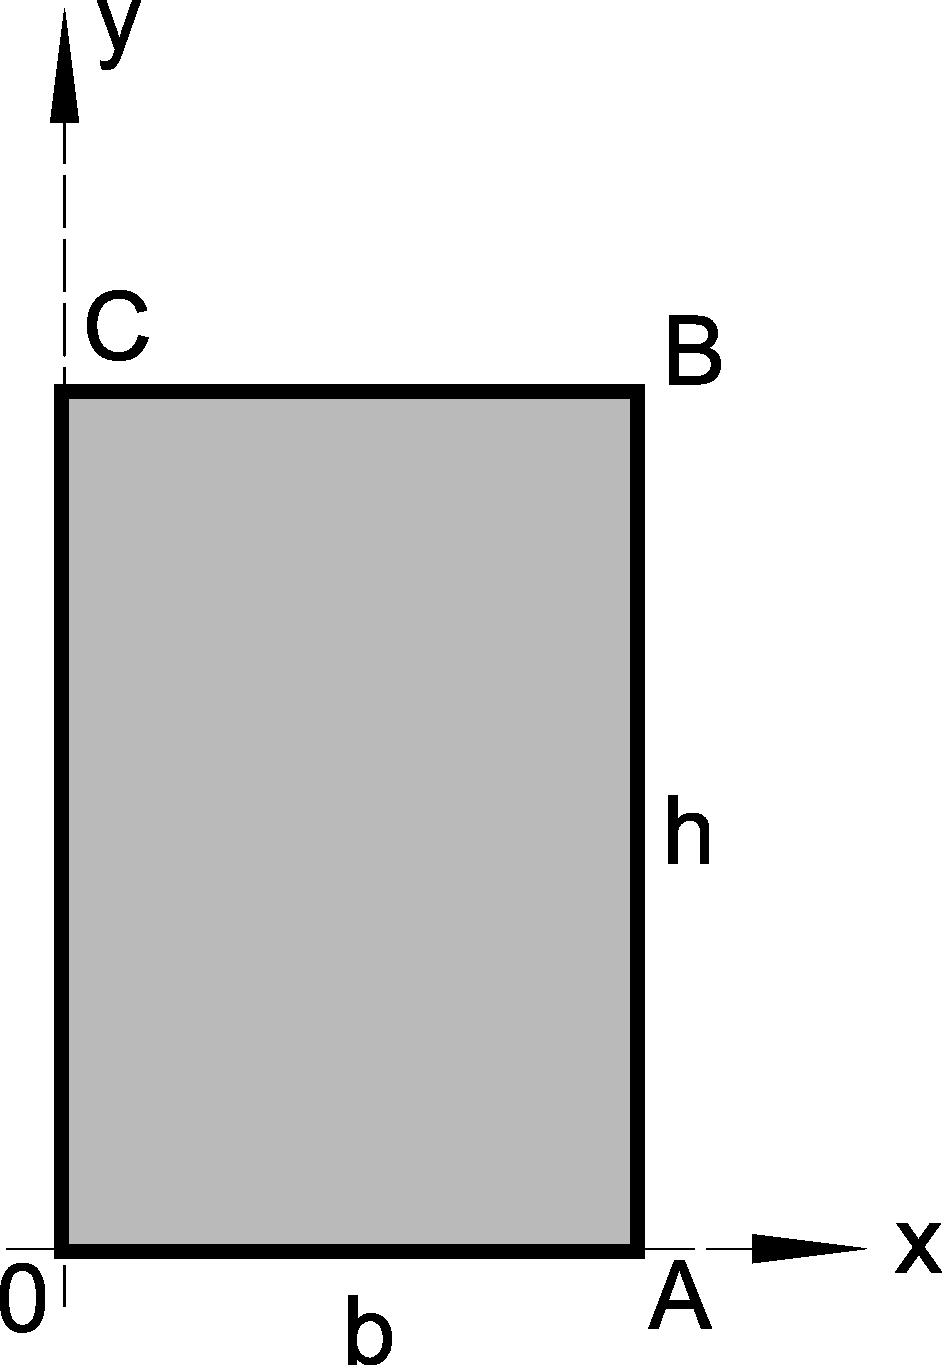
\includegraphics[scale=0.25]{Rectangulo.pdf}
		\caption{Rectangulo en la configuraci\'on no deformada}
		\label{Rectangulo}
	\end{figure}

Se pide determinar lo siguiente:
	
\begin{enumerate}
	\item Calcular los desplazamientos de los puntos $A$, $B$ y $C$ para cada uno de los estados de deformaci\'on y dibujar las configuraciones deformadas.
	\item Si se sabe que las dimensiones del rect\'angulo $b=1.00$ y $h=1.00$ y los valores de las transformaciones son $d=0.01$, $e=0.005$ y $f=0.0025$. Calcular las direcciones principales y los valores propios para la superposici\'on lineal de las deformaciones. 	
\end{enumerate}

\newpage
\item  \label{punto04_d} En la figura \cref{BarraColgada} se muestra una barra de sección circular de radio $R$, altura H, soportada de su extremo superior y que está sometido solamente a la acción de su peso propio. El campo de desplazamientos $u,v,w$ en el sistema coordenado $xyz$ de para la barra está dado por: \\

	$u= -\nu \dfrac{\gamma}{E} z x $ \hspace{1cm}	
	$v= -\nu \dfrac{\gamma}{E} z y $ \hspace{1cm}	
	$w= \dfrac{\gamma}{2E} z^2 +\dfrac{\gamma \nu}{2E} (x^2+y^2)-\dfrac{\gamma}{2E} H^2  $ \\
	
donde $E$, $\gamma$ y $\nu$ son constantes del material (posititivas). 
	
\begin{figure}[H]
	\centering
	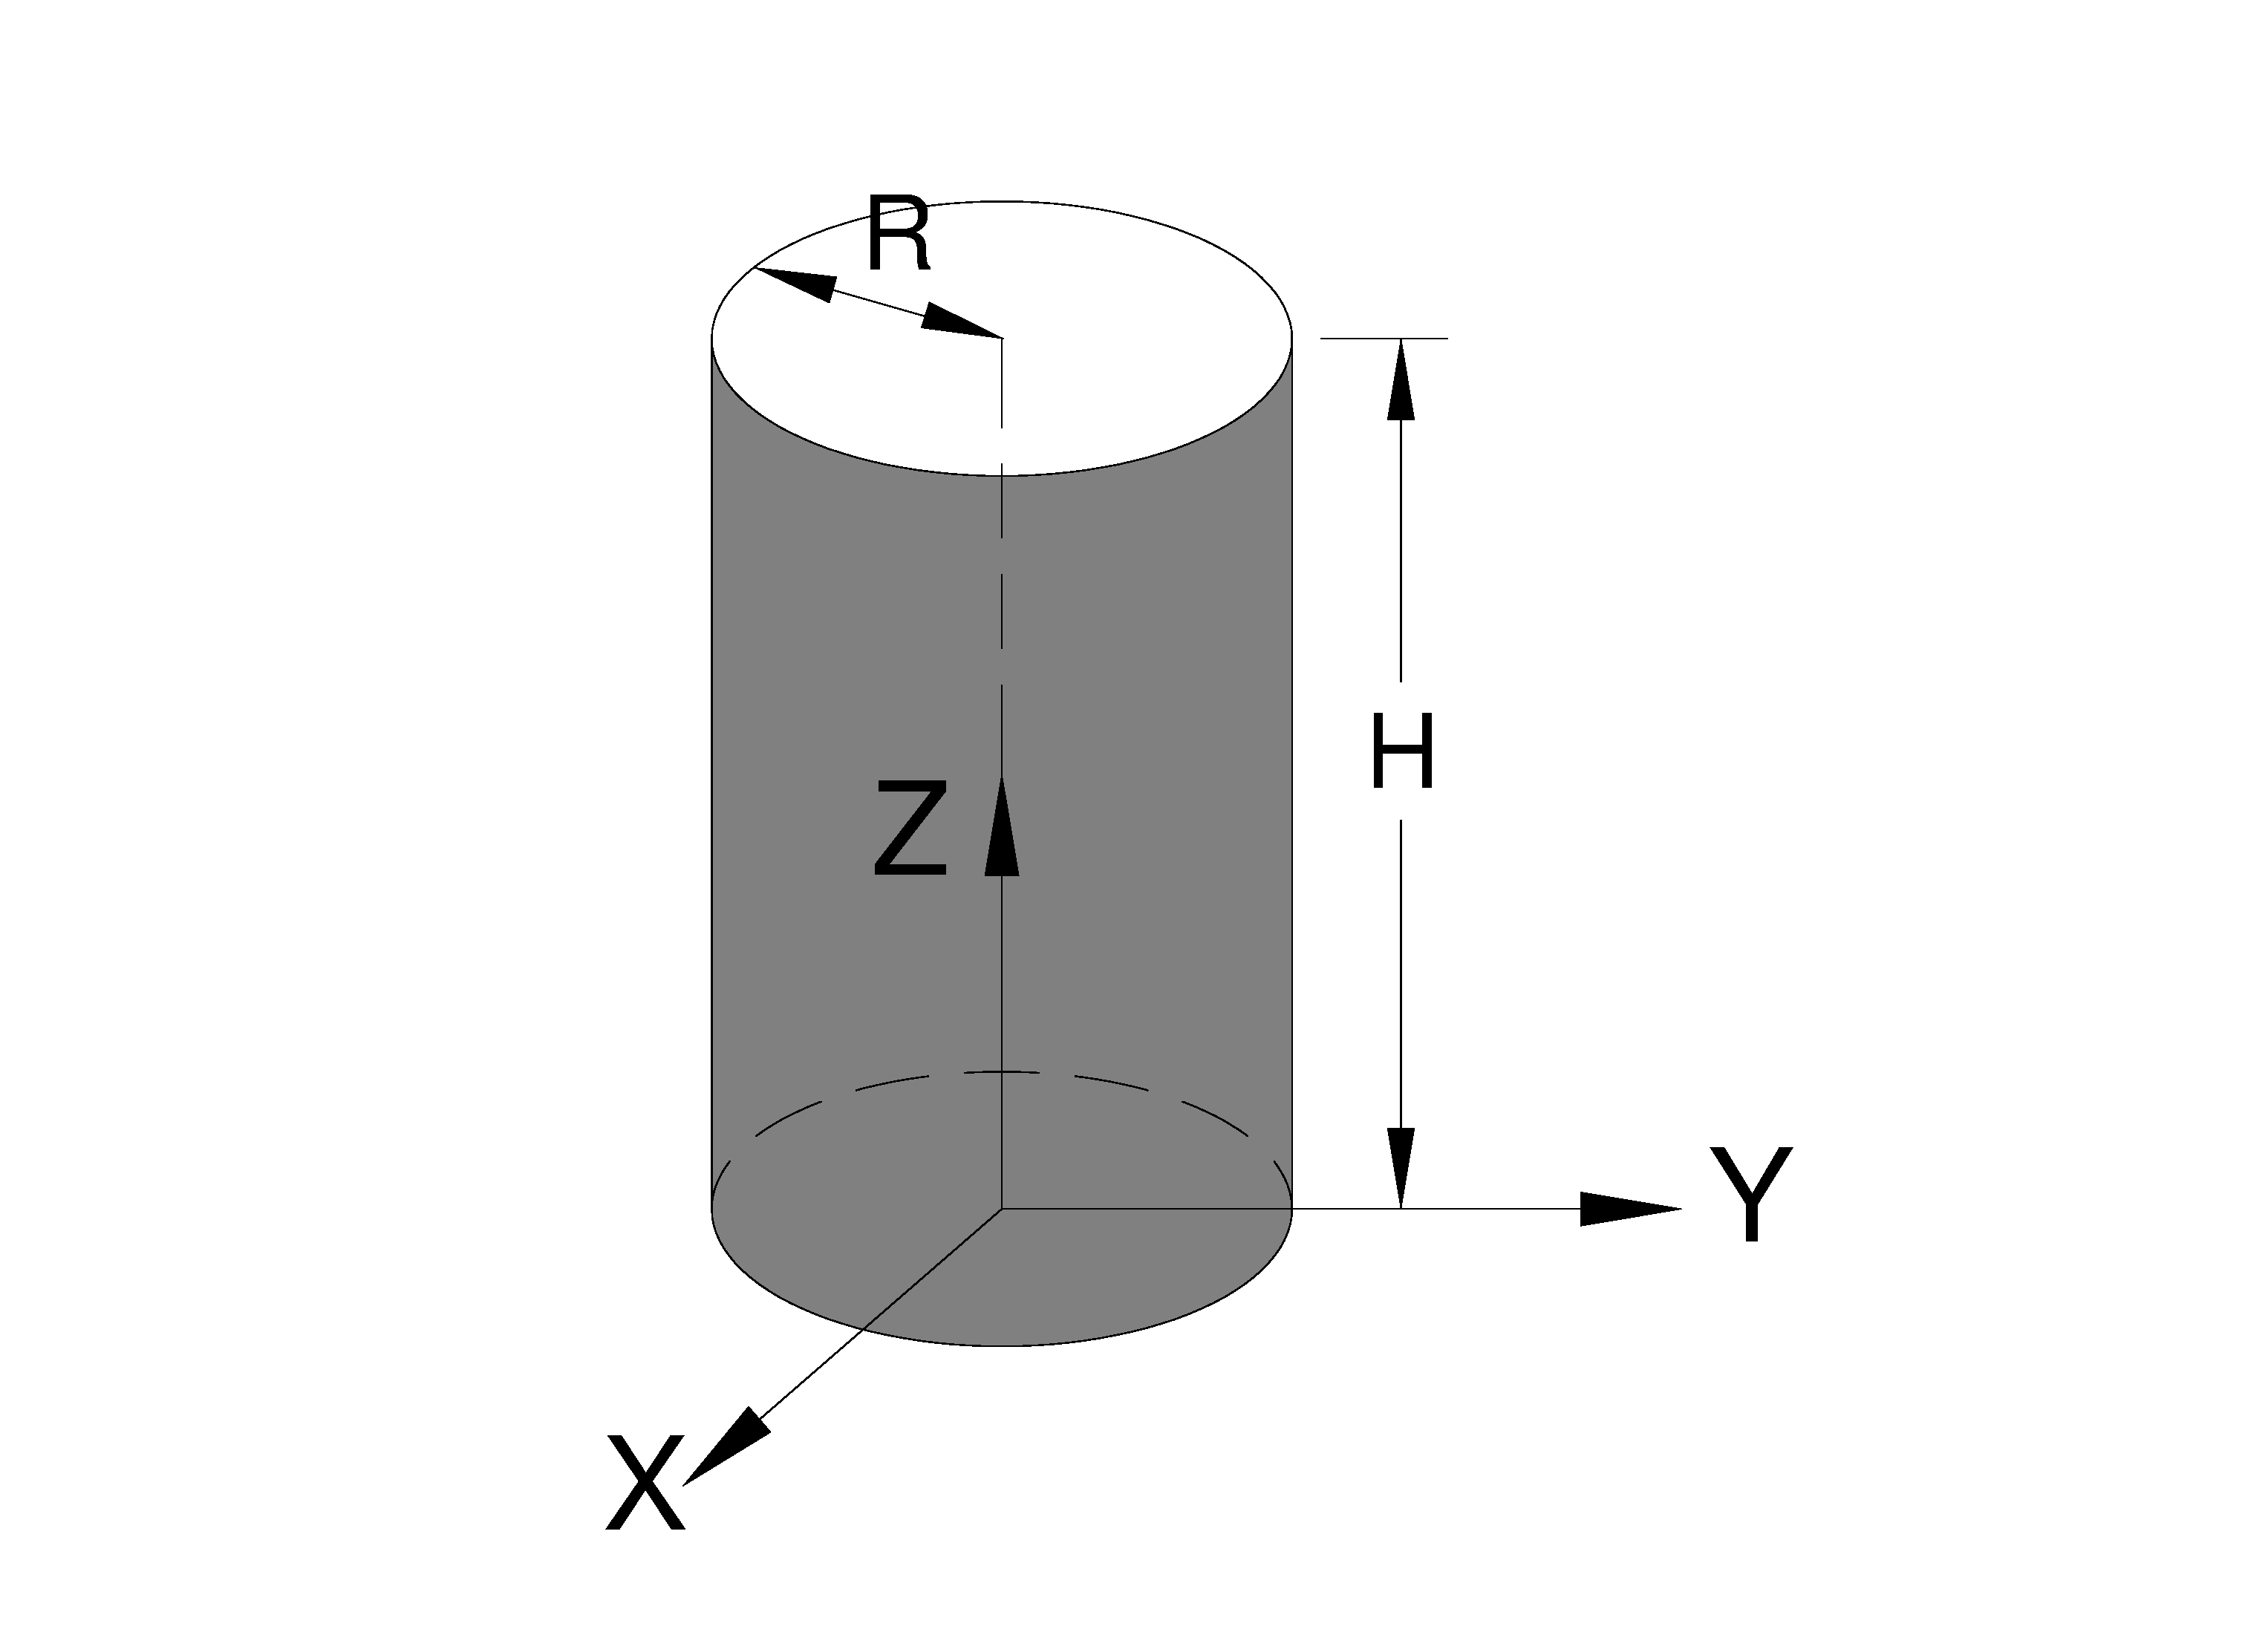
\includegraphics[height=6cm]{barracolgada.pdf} \label{figure1}
	\caption{Barra colgada}
	\label{BarraColgada}
\end{figure}
%
\begin{enumerate}
% 
	\item Esboce la configuraci\'on deformada de la barra.	
	\item Calcule el tensor de deformaciones y descompóngalo en su componente simétrica: $[\varepsilon]$ y asimétrica  $[\omega]$
	\item Cuáles son los valores máximos y mínimos de las deformaciones axiales, $\varepsilon_{xx}$, $\varepsilon_{yy}$, $\varepsilon_{zz}$, y en que puntos se presentan.
	\item Cuáles son los valores máximos y mínimos de los desplazamientos: $u$, $v$, $w$ y en que puntos se presentan.
	\item ¿ Existen puntos exentos de rotaci\'on de cuerpo r\'igido?, responda s\'i o no y justifique su respuesta.	
	\item ¿ Es posible encontrar puntos sometidos a distorsi\'on angular?, responda s\'i o no y justifique su respuesta.
%
\end{enumerate}
%
\newpage

\item  \label{punto05_d}  En la figura \cref{VigaMomentoflec} se muestra un medio continuo de sección rectangular de ancho unitario, altura $H$, soportado en un extremo ($X = 0$), y sometido en su otro extremo ($X = L$) a la acci\'on de un momento flector $M$ alrededor del eje $Z$. Si el campo de desplazamientos en el sistema coordenado $XYZ$ est\'a dado por: \\

	$u= -\dfrac{M}{EI} X Y $ \hspace*{10mm}	
	$v= \dfrac{M}{2EI}(X^2+ \nu (Y^2-Z^2)) $ \hspace*{10mm}	
	$w= \dfrac{\nu M}{EI} Y Z  $\\


Donde $u,v,w$ son los desplazamientos asociados a los ejes $X,Y,Z$ respectivamente. $E$ y $\nu$ son constantes  (positivas) del material e $I$ es el momento de inercia alrededor del eje Z de la secci\'on tranversal. \\ 
\begin{figure}[H]
	\centering
	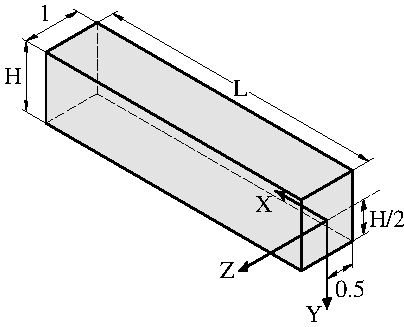
\includegraphics[height=6cm]{VigaMomento.pdf}
	\caption{Viga sometida a momento flector}
	 \label{VigaMomentoflec}
\end{figure}
%
\begin{enumerate}
\item En la figura \cref{ConfiguraFlector} se muestran esbozos de posibles configuraciones deformadas (secci\'on achurada) de la viga mostrada en la figura \label{VigaMomento}. Determine en cada caso cual es la configuración correcta. 
%
\begin{enumerate}
%
	\item[•] Para la secci\'on transversal en $X = L$. 
	\item[•] Para una secci\'on longitudinal cuando $Y > 0$.
	\item[•]  Para una secci\'on longitudinal asociada al plano ($Y = -H/2$)
	\item[•]  Para una secci\'on longitudinal asociada al plano ($Z = 0$) 
%
\end{enumerate}
%
\begin{figure}[H]
	\centering
	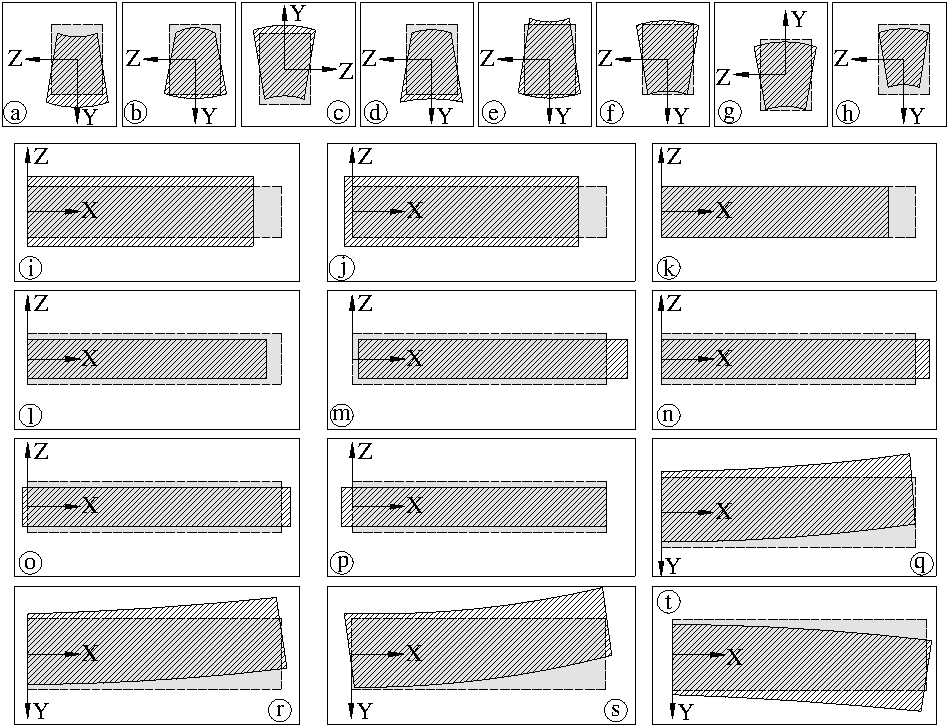
\includegraphics[height=12.00cm]{Configuracion.pdf}
	\caption{Posibles configuraciones deformadas de secci\'on transversal}
	\label{ConfiguraFlector}
\end{figure}
%
\item Calcule el tensor de deformaciones  $[\varepsilon]$ y el de rotación $[\omega]$ 
\item Si el valor de la distorsi\'on angular m\'axima es $\gamma$ = $\gamma_{max}$ determine cual es el momento m\'aximo posible, $M_{max}$ que podría ser aplicado. 
\item¿Cu\'ales son las coordenadas $x,y,z$ de los puntos que experimentan mayores rotaciones de cuerpo r\'igido?
\item ¿Cu\'ales son los puntos que experimentan la menor rotaci\'on de cuerpo r\'igido? 
\item Cuales son los valores m\'aximos y m\'inimos de las deformaciones axiales, $\varepsilon_{xx}$, $\varepsilon_{yx}$, $\varepsilon_{zz}$ y en que puntos se presentan.
\item Cu\'ales son los valores m\'aximos y m\'inimos de los desplazamientos, $u$, $v$, $w$, y en que puntos se presentan.
\item ¿Existen puntos exentos de rotaci\'on de cuerpo r\'igido?, responda s\'i o no y justifique su respuesta.
\item ¿Es posible encontrar puntos sometidos a distorsi\'on angular?, responda s\'i o no y justifique su respuesta.
%
\end{enumerate}
%
\newpage

\item \label{punto07_d}  En la figura \cref{Solucion_Flamant} se  muestra la solución de un semi-espacio sometido a una carga lineal superficial $P$.  Los desplazamientos al interior del suelo debidos a la carga P est\'an dados por:  \\\\
%
%\begin{large}
	\hspace*{10mm} $ u_r (r,\theta) = -\dfrac{2P}{\pi{E}} \ln{r}$ ${\cos \theta} -\dfrac{(1 - \nu)P}{\pi{E}} {\theta}$ $ {\sin\theta} + B $ $ {\cos \theta} $ \\\\
	\hspace*{10mm} $ u_{\theta}(r,\theta) = \dfrac{2{\nu}P}{\pi{E}} \sin\theta + \dfrac{2P}{\pi{E}}\ln{r}$ $\sin\theta -\dfrac{(1 - \nu)P} {\pi{E}} 
	{\theta}$ $ {\cos\theta} + \dfrac{(1 - \nu)P}{\pi{E}}$ ${\sin\theta} - B$ $ {\sin\theta}$	\\\\
	\hspace*{10mm} $ w (r,\theta) = 0$ \\\\
%%\end{large}
%
\noindent Donde $E$ es el m\'odulo de elasticidad,  $\nu$ es la relaci\'on de Poisson del material y $B$ es una constante positiva.
%
\begin{figure}[H]
	\centering
		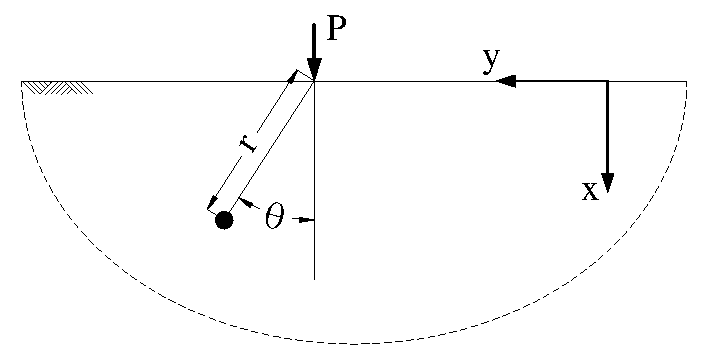
\includegraphics[height=3.0cm]{Flamat.pdf} 
		\caption{Soluci\'on carga vertical}
		\label{Solucion_Flamant}
\end{figure}
%
Si en un suelo sometido a la acción de dos estructuras que le transmiten  una carga lineal superficial, $P$ y $3P$, respectivamente tal como se muestra en la figura  \cref{figure3} se desea instalar una tuber\'ia, perpendicular al plano mostrado ($XY$), de di\'ametro despreciable, en el punto indicado  en la figura \cref{figure3}.
%		
\begin{figure}[H]
	\centering
	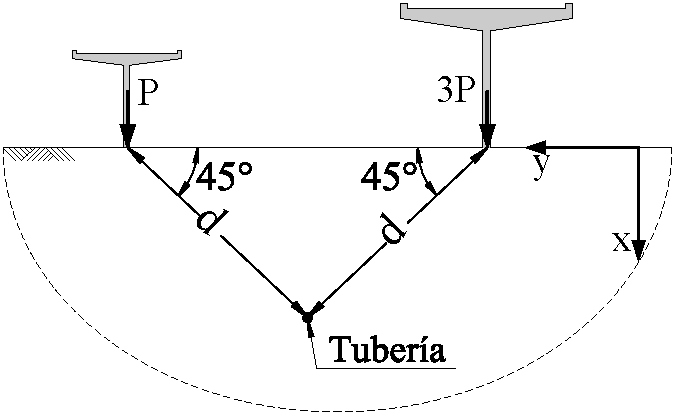
\includegraphics[height=3.2cm]{ProblemTub.pdf} 
	\caption{Estructuras y tuber\'ia.}
	\label{figure3}
\end{figure} 
\begin{enumerate}
%
	\item Determine cuál es el valor de la deformación axial máxima.
	\item  Si la m\'axima deformaci\'on angular a la que puede ser sometida la tuberia sin fallar, es igual a: $\gamma_{max}$. ¿Cu\'al es el m\'aximo valor de la carga distribuida $P$ que pueden transmitir las estructuras para que la tuber\'ia no falle?. 
	\item Esboce la configuraci\'on deformada de la part\'icula correspondiente al punto donde se ubica la tuber\'ia. Solo considere el plano $xy$. 
\end{enumerate}
\newpage
\item \label{punto08_d} En la figura \cref{BarraApoya} se muestra una barra de radio $R$ y longitud $L$. El campo de desplazamientos   en el sistema coordenado $xyz$, est\'a dado por:\\
\\
\begin{large}
	\hspace*{20mm} $u= -\theta yz$, \hspace*{35mm} $v= \theta xz $, \hspace*{35mm}
	$w= 0  $\\
\end{large}
%
\\
%
Donde $u,v,w$ son los desplazamientos asociados a los ejes $x,y,z$ respectivamente. $\theta$ es una constante positiva. \\ 
\begin{figure}[H]
	\centering
	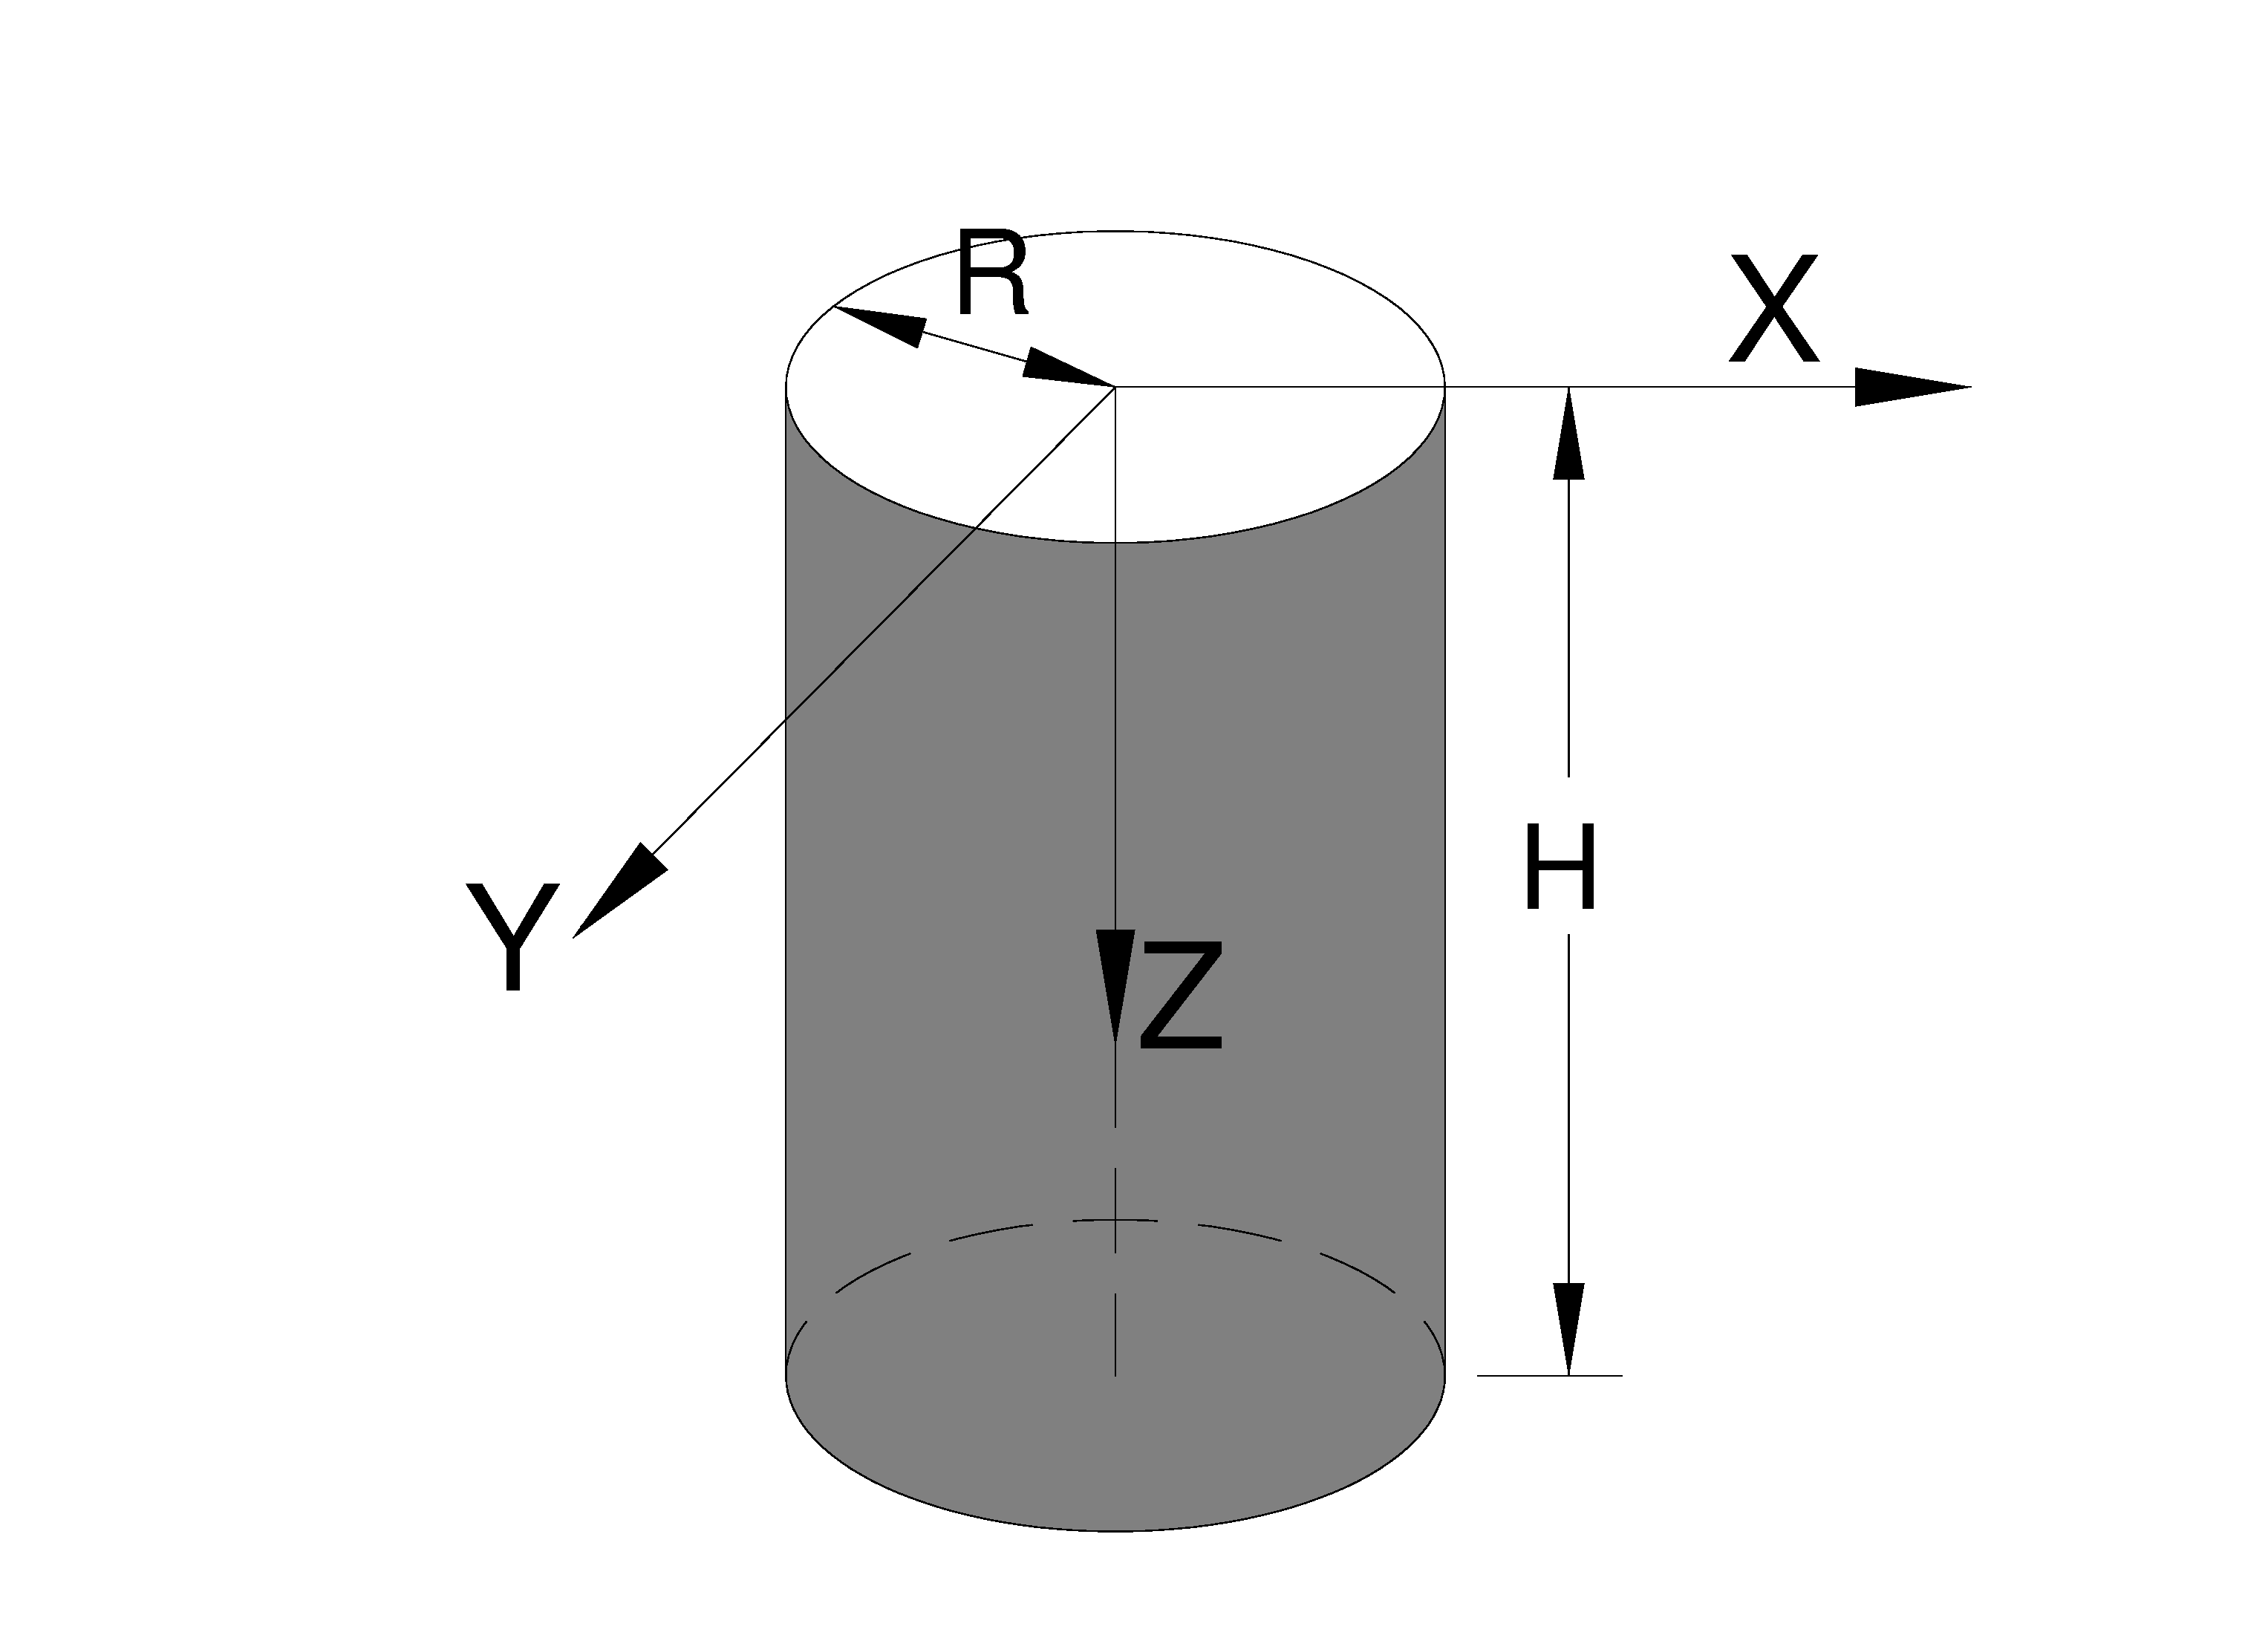
\includegraphics[height=5cm]{barraapoyada.pdf} 
	\caption{Medio Continuo}
	\label{BarraApoya}
\end{figure}

\begin{enumerate}

\item Dibuje la configuraci\'on deformada de la barra. 
%
\item Calcule el tensor de deformaciones, $[D]$, y determine: tensor de deformaci\'on $[\varepsilon]$ (sim\'etrico) y tensor de rotaci\'on $[\omega]$ (asim\'etrico).
\item Ilustre la deformaci\'on de la part\'icula en el punto de coordenadas $y = R$ y $x = 0$. Para la ilustraci\'on use cuadrados de tama\~no diferencial contenidos en los planos $xy$, $xz$, $yz$ de forma independiente. En la ilustraci\'on debe incluirse los efectos de cuerpo r\'igido.
\item ¿ Cu\'ales son los puntos que experimentan mayores rotaciones de cuerpo r\'igido?
\item Cu\'ales son los valores m\'aximos y m\'inimos de los desplazamientos, $u$, $v$, $w$ y en que puntos se presentan:
\item  \textquestiondown Es posible encontrar puntos sometidos a distorsi\'on angular?, responda s\'i o no y justifique su respuesta.
%
\end{enumerate}

\newpage

\item  \label{punto09_d} En la figura \cref{cuna} se presenta una cu\~na de espesor $t$ sometida a la acci\'on de una carga (en el plano $XY$) distribuida sobre su per\'imetro.
%
\begin{figure}[H]
	\centering
	{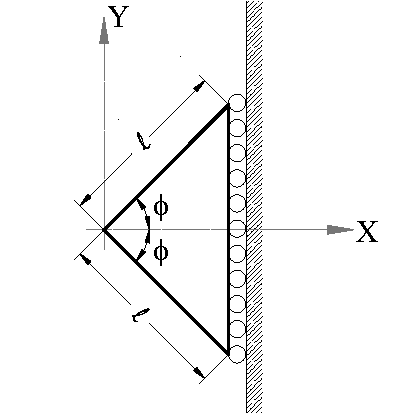
\includegraphics[width=8cm]{Cunasup.pdf}}\
	\hspace{2 cm}
	\caption{Cu\~na de espesor $t$}
	\label{cuna}
\end{figure}
%
El campo de desplazamientos de la cu\~na  esta dado por:\\\\
%
%\begin{large}
	\hspace*{10mm} $ u(x,y) = \dfrac{2B}{E} (\cot \phi + \nu \tan \phi) (x - l\cos \phi) $
	\hspace*{10mm} $ v(x,y) = - \dfrac{2B}{E} (\tan \phi + \nu \cot \phi) y$	
%\end{large}

\hspace*{10mm} Donde $B$, $E$ y $\nu$ son constantes positivas. \\\\
%
Adem\'as, se sabe que:\\\\
%
 $\sigma_{xx} = \dfrac{E}{(1 - \nu^2)} (\varepsilon_{xx} + \nu \varepsilon_{yy}) $ 
\hspace*{5mm} $\sigma_{yy} = \dfrac{E}{(1 - \nu^2)} (\varepsilon_{yy} + \nu \varepsilon_{xx}) $ 
\hspace*{5mm} $\tau_{xy} = \dfrac{E}{2(1 + \nu)} \gamma_{xy} $\\\\
%
\begin{enumerate}
	%
	\item Dibuje la configuraci\'on deformada de la cu\~na. 
	\item Ilustre la deformaci\'on de la part\'icula en el punto de coordenadas $X = 0$ y $Y = 0$. En la ilustraci\'on deben incluirse los efectos de cuerpo r\'igido. 	
    \item Si $\nu=0.25$ y $\phi=53.13^{\circ}$, determine la reacciones (Fuerzas) en el soporte .\\\\\\
	%
\end{enumerate}

\newpage
%
%
\item  \label{punto10_d} Si el campo de desplazamientos para la barra mostrada en la \ref{def:Mario} est\'a dado por:\\\\
%
	$u\left( x \right) = -\dfrac{1-\nu^2}{E} \sigma_0 x$, \hspace*{10mm} $v=0$, \hspace*{10mm} $w\left( z \right) = \nu \dfrac{1+\nu}{E} \sigma_0 z$

\begin{figure}[H]
	\centering
	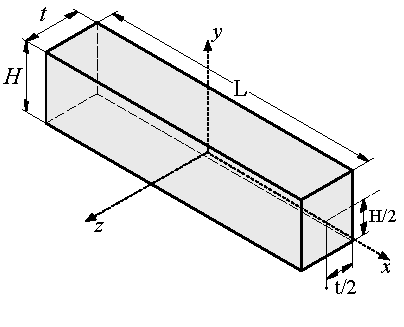
\includegraphics[height=5cm]{Viga.pdf} 
	\caption{Viga de Longitud $= L$, Altura $=H$ y Espesor $=t$. El origen del sistema coordenado coincidiendo con el centroide de la barra.}
	\label{def:Mario}
\end{figure}

\begin{enumerate}
%
	\item Explique a que acciones externas está sometida la barra
	\item Dibuje la configuracio\'on deformada de la barra
	\item \textquestiondown Hay partículas sometidas a rotaciones de cuerpo rigido? (responda s\'i o no y justifique su respuesta).
	\item \textquestiondown Hay partículas que {\textbf{NO}} experimenten distorsiones angulares? (responda si o no y justifique su respuesta).
	\item En que coordenadas está la part\'icula que sufre mayor deformaci\'on axial y cu\'al es el valor de esta deformaci\'on.
	\item En que coordenadas est\'a la part\'icula que sufre mayor distorsi\'on angular y cu\'al es el valor de esta deformaci\'on.
	\item Encuentre los desplazamientos y deformaciones del punto de coordenadas $\left( 0,0,0 \right)$.
%
\end{enumerate}
%
% **** Punto 11
% ***** Empieza modelos constitutivos
\item   \label{punto11_d} Para un campo de desplazamientos dado por:
\[\mathbf{u} = a(x^2 - 5y^2)\hat{\mathbf{i}} + (2ax y)\hat{\mathbf{j}} \]

\begin{enumerate}
\item Determinar el tensor de deformaci\'on;
\item Obtener las deformaciones principales;
%\item Dado el m\'odulo de cortante $G$ \textquestiondown qu\'e valor toma el m\'odulo de Young $E$ para que haya equilibrio en cualquier punto?
\end{enumerate}

\newpage

\item \label{punto12_d} En la figura \cref{fig:barra} se presenta una barra sobre la cual se aplica una fuerza en dirección $x$ $F_{x}$, que genera  un esfuerzo constante $\sigma_x$ sobre la sección transversal donde está aplicada. La barra inicialmente está  separada de una lámina delgada de acero una distancia $d$ tal y como se muetra en \cref{sfig:barra2D}. El campo de desplazamientos para la barra mostrada está dado por:\\\\
%
\hspace*{20mm} $u\left( x \right) = \dfrac{1}{E_1}  x \sigma_x$, \hspace*{10mm} $v=0$, \hspace*{10mm} $w\left( z \right) = - \dfrac{1}{E_2}  z (H^2 - y^2) \sigma_x$ \\

Donde $E_1 = 200000 kgf/cm^2$,   y $E_2 = 1000000$ $kgf/cm^4$, $L = 1000 cm$, $H= 10 cm$.   $\sigma_x$ es el esfuerzo en dirección $x$ el cual tiene una variación en el tiempo deacuerdo a como lo muestra la  \cref{sfig:stress}.  

\begin{figure}[H]
	\centering
		\subfloat [Configuración inicial de la barra en 3D. Aplicación de la fuerza]{ 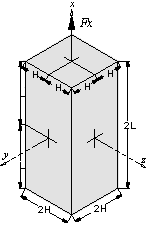
\includegraphics[width=1.6in]{Barra.pdf}\label{sfig:barra3D}}
		\hspace{0.7cm}
		\subfloat [Vista plano $xz$. Separación inicial barra - lámina, d = 2.0 cm. $\phi = 45^\circ$.]{ 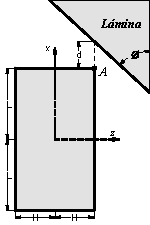
\includegraphics[width=1.6in]{BarraPared.pdf}\label{sfig:barra2D}}
		\hspace{0.7cm}
		\subfloat [Curva de esfuerzo.]{ 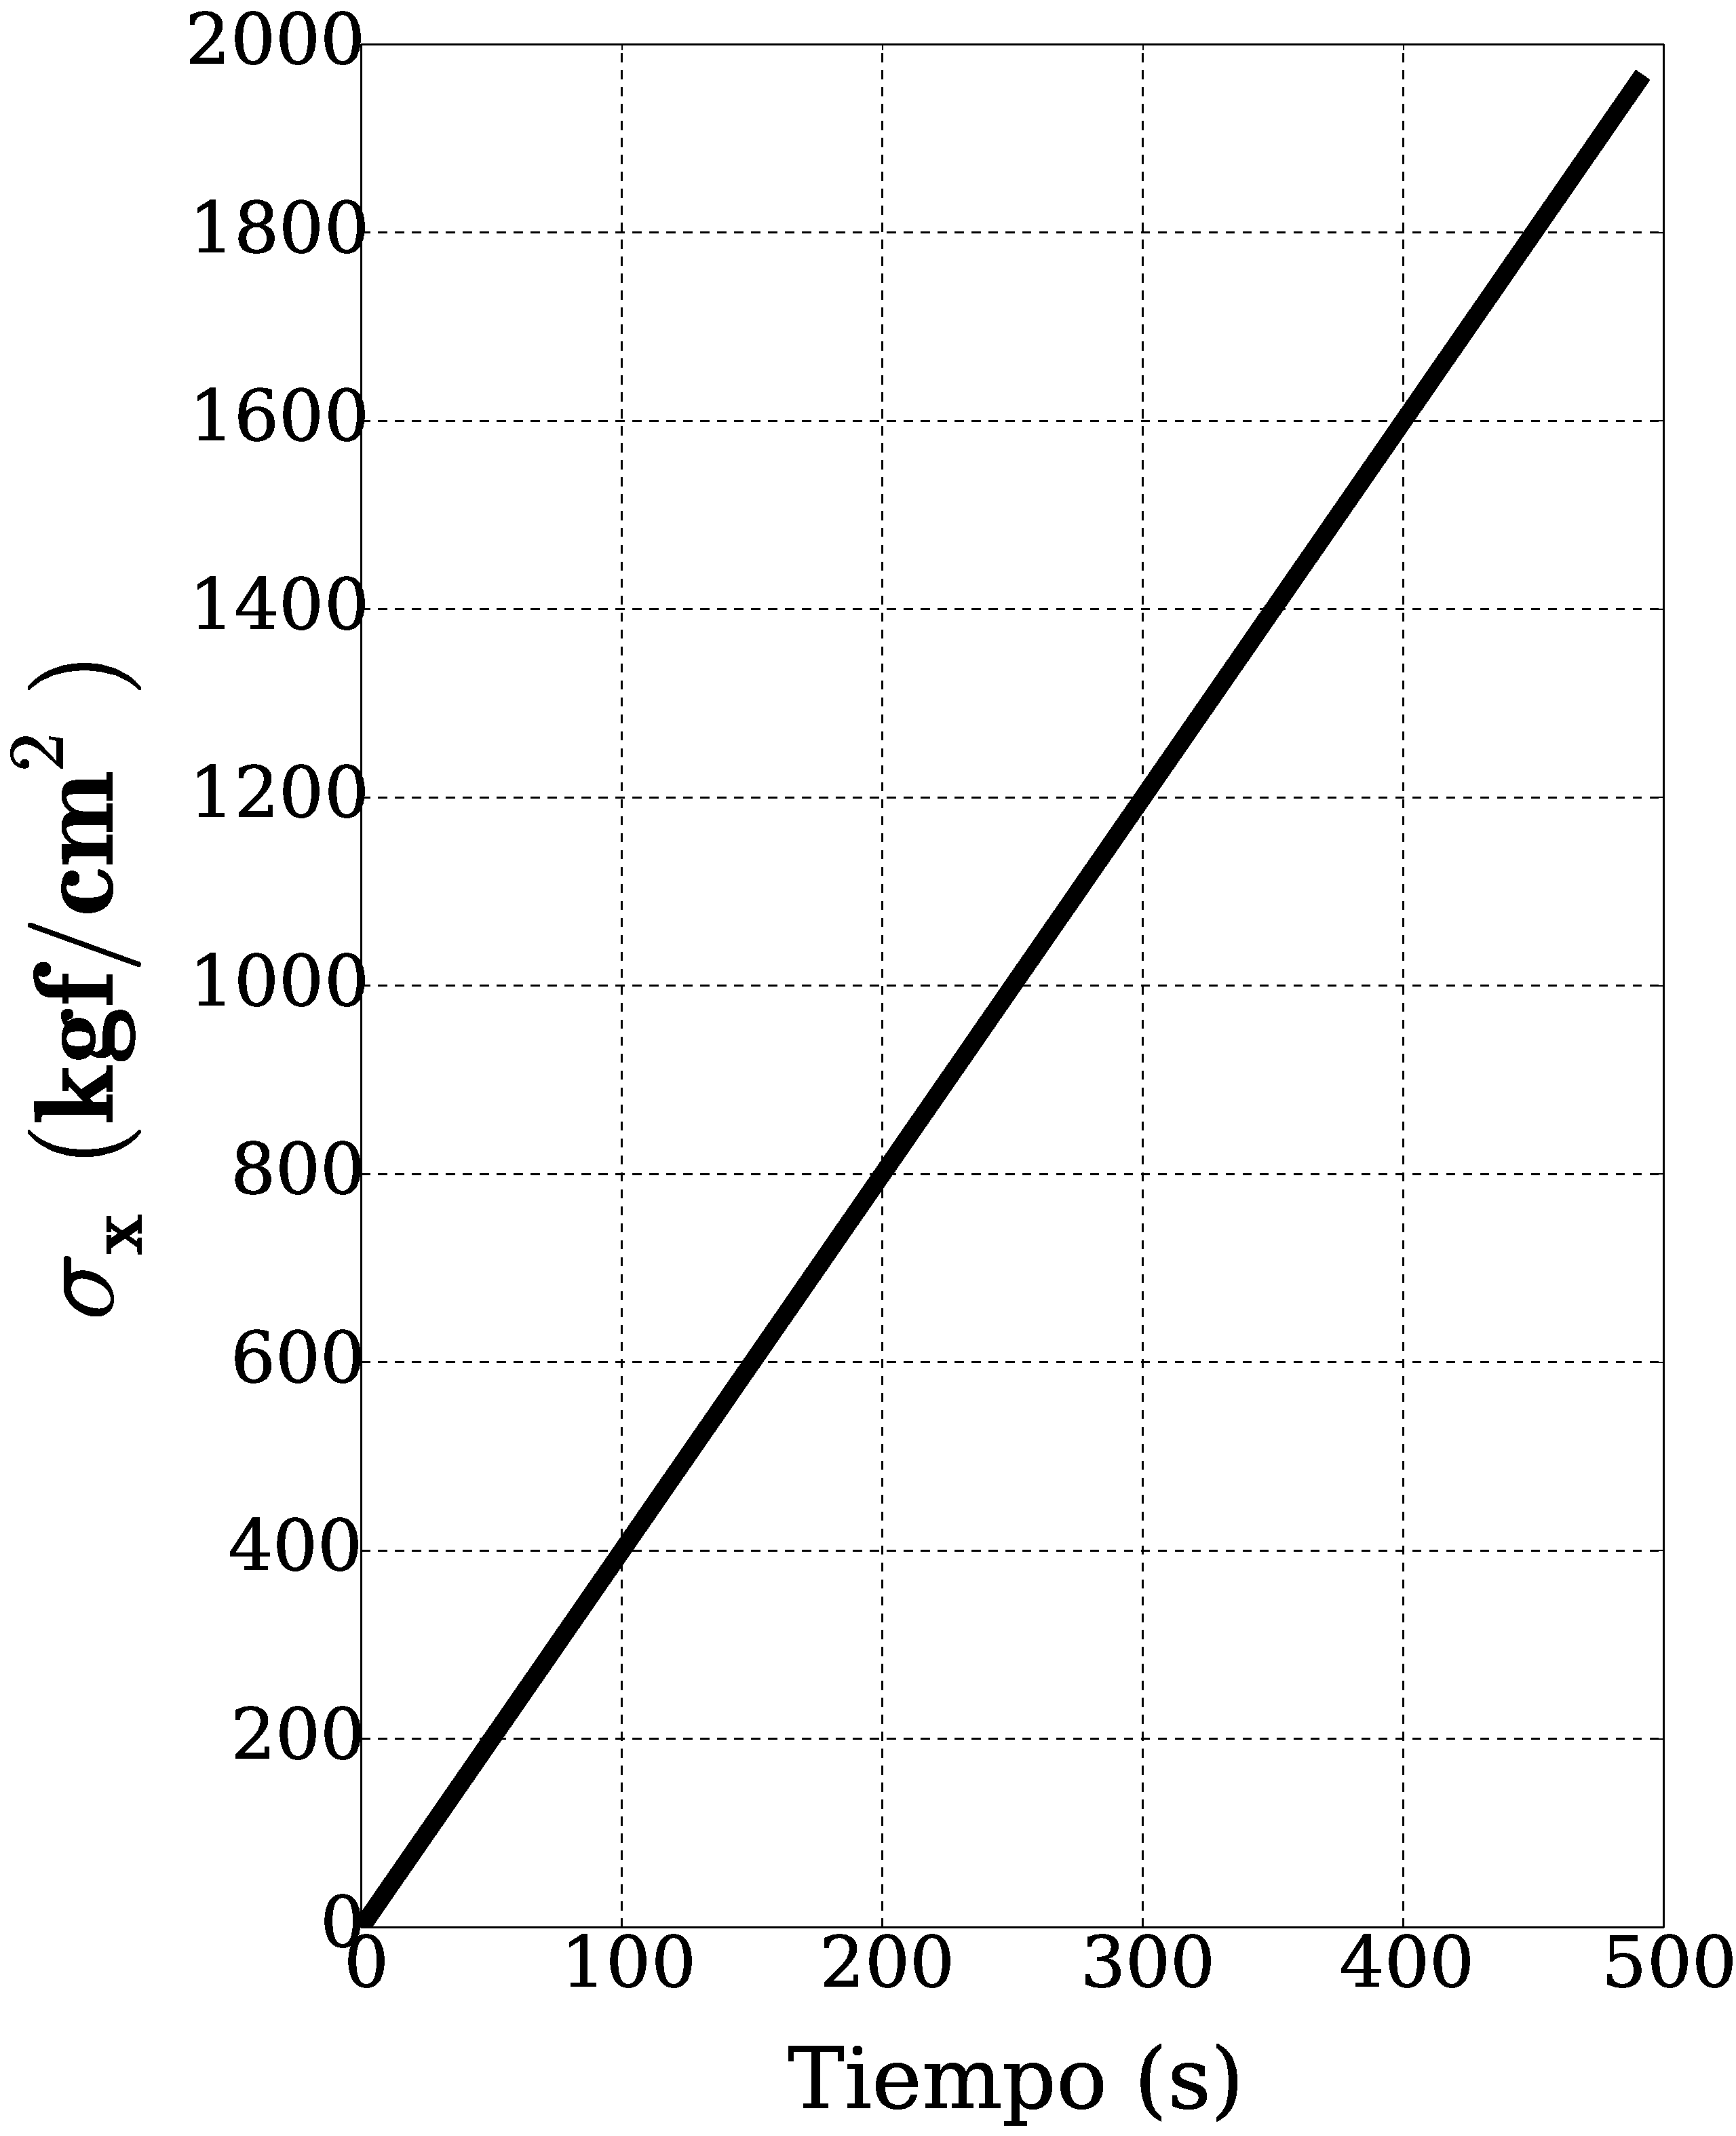
\includegraphics[width=1.9in]{CurvaEsf.pdf}\label{sfig:stress}}			
	\caption{Barra sometida a fuerza axial $F_{x}$}
	\label{fig:barra}
\end{figure}


\begin{enumerate}
	%
	\item Para el punto A de la barra con coordenadas  $(x,y,z) = (L, 0, B)$ grafique los desplazamientos $u$ y $w$ en función de tiempo. 
	\item Dibuje la configuración deformada de la partícula para el punto de coordenadas $(x,y,z)=$ $(0,0,0)$ 
	\item  Si el valor de $\sigma_x = 50  kgf/cm^2$ y se estudian solo los puntos de la cara $ z = 1.0 cm$ determinar el valor de la distorsión angular máxima y las coordenadas $x,y,z$ de los puntos  en que se presenta. 	
	\item Si el esfuerzo  $\sigma_x$ se incrementa  hasta que el punto  $A$ con coordenadas  $(x,y,z) = (L, 0, B)$ toque la lámina, determine el tiempo $t$  en el que la barra toca la lámina. ¿Cuáles serían las coordenas finales $x$, $z$ del punto A en ese instante?

\end{enumerate}


\item  \label{punto13_d}  En un ensayo de un elemento de concreto se mide la deformación en un mismo punto mediante tres galgas de deformación. Las galgas de deformación se disponen en un arreglo tal y como se muestra en la \cref{ensayogalga},

	%
	\begin{figure}[H]
		\centering
		\hspace*{6mm}
			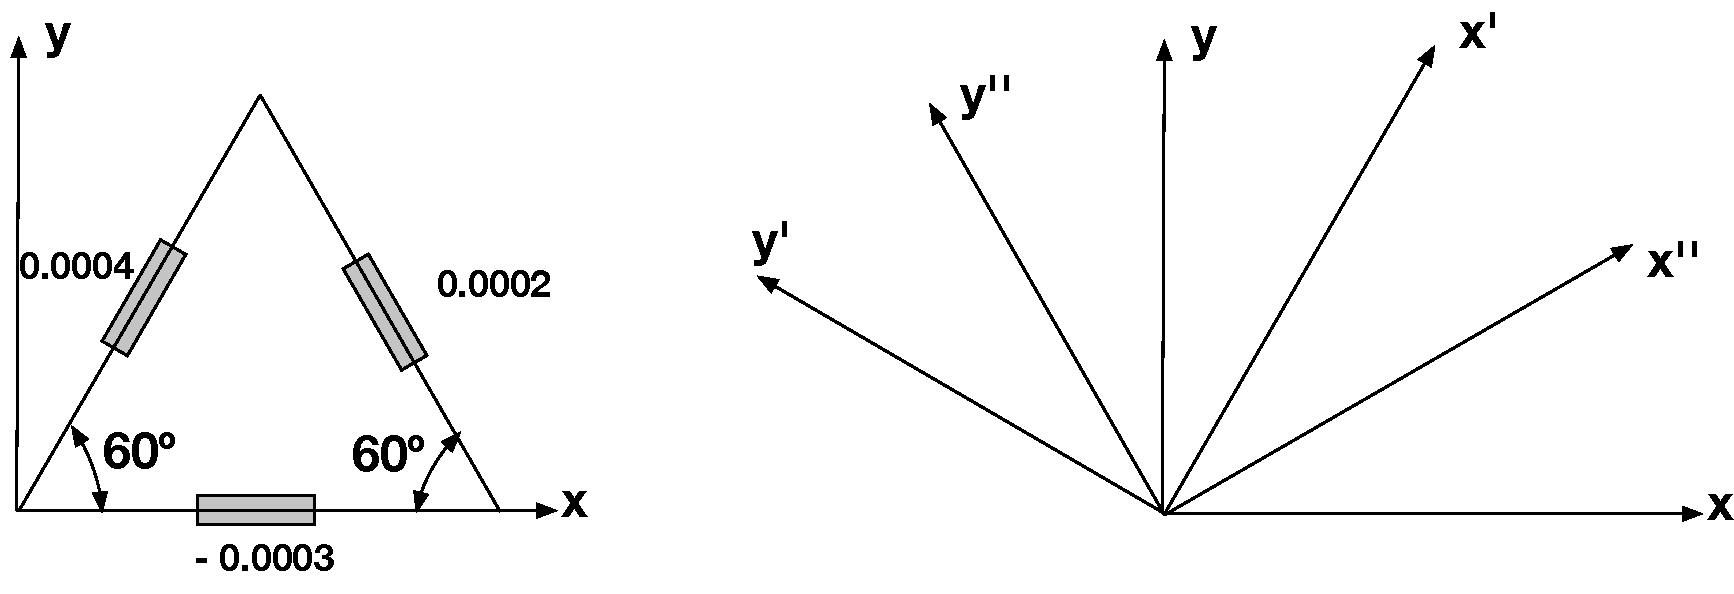
\includegraphics[width=4.5in]{galgas.pdf}
		\caption{ Galgas de deformación}
		\label{ensayogalga}
	\end{figure}
	%

Si las galgas solo registran la deformación axial y las mediciones de laboratorio reportaron: $\varepsilon_{xx} = -0.0003$; $\varepsilon_{x'x'} = 0.0004$; $\varepsilon_{y''y''} = 0.0002$. Se solicita

\begin{enumerate}
\item Tensor de deformaciones en el sistema $xy$, $x'y'$ y $x''y''$. 

\item Distorsión angular máxima. 

\item Deformación axial máxima

\item Configuración deformada de la partícula
\end{enumerate}

\end{enumerate}

\end{document}


